\chapter{Discovering Hydrothermalism from Afar}
\label{chap:afar}

\begin{center}
    \begin{minipage}{0.7\textwidth}
      \begin{small}
      I had a blank canvas to fill with extraordinary possibilities, a fascinating jigsaw puzzle to piece together: mapping the world's vast hidden seafloor.\\ \emph{Marie Tharp}
      \end{small}
    \end{minipage}
    \vspace{0.5cm}
\end{center}

To track a spatiotemporal phenomenon requires first being able to sense it. There are two core challenges associated with perceiving hydrothermal plumes: existence (and availability) of technology and interpretation of heterogeneous data streams. With respect to deep-sea capable instrumentation, temperature, pressure, conductivity, and turbidity are all examples of quantities that can be near instantaneously measured by existing state-of-the-art \emph{in situ} sensors. However, for many geochemical quantities such as dissolved greenhouse gases (e.g., carbon dioxide, methane), few (if any) commercial sensors with rapid response times suitable for use on a mobile platform exist. This limitation has had severe impact on the ability for scientists to study phenomena like hydrothermal plumes, as these entities may be difficult to identify only from temperature or conductivity anomalies, but are expected to be significantly geochemically distinctive from background seawater levels of the ocean \autocite{scholz2019shelf,jakuba2007stochastic}. In this chapter, two experimental dissolved methane instruments are used in an ocean trial at a hydrothermal basin. The utility of methane as a signal for the presence of plume waters is compared against other standard oceanographic equipment.

The second challenge, interpreting heterogeneous data streams, is a problem that arises when the quantity of interest is a conceptual entity, rather than an absolute one. Concretely; temperature can be directly observed with a single instrument, but ``plumes'' cannot be directly sensed as they are by definition an aggregation of properties distinct from background seawater. So, to observe ``plumes'' requires interpreting data from multiple heterogeneous sensors in order to identify which robot locations observed plume-derived fluids, and which did not. Heterogeneity in this case refers to the different operating principles and observable quantities that are measured by a suite of scientific sensors. As these sensors may respond to the environment at different time scales, have different sensitivities, and measure quantities which may physically manifest themselves differently in unique spatiotemporal regions of a plume (and may be unique to each plume that is surveyed), it is not straightforward to universally filter these data streams for plume detections. To this end, this chapter presents several methods for detecting ``change-points'' in data streams that can be used to indicate anomalous features in a data stream unique to hydrothermalism, and which can be broadly applied to many different types of field settings.

The content that proceeds from this point is directly adapted from~\cite{preston2022discovering}, which was published in Frontiers Earth Science in 2022. The supplemental information for this publication is also reproduced as Appendix~\ref{app:perception} in this thesis.


\section{Introduction}
Detecting and characterizing seafloor hydrothermal vents is critical in understanding the fundamental interactions among the geochemical and biological processes on the seafloor, and the fluxes that these processes cause to and from the deep ocean. Since the first discovery of deep sea hydrothermalism in 1977 \autocite{corliss1979submarine}, hundreds of hydrothermal venting sites have been discovered and analyzed \autocite{beaulieu2015undiscovered}. These studies reveal that hydrothermal vents play a major role in ocean-scale elemental and micronutrient budgets \autocite{le2019hydrothermal,resing2015basin}, serve as nutrient pumps to the deep ocean \autocite{dick2013microbiology, vic2018dispersion, scholz2019shelf, bell2017hydrothermal}, and sustain abundant and unique (e.g., chemosynthetic) forms of complex life \autocite{grassle1987ecology, georgieva2021history}. Hundreds more vent sites are hypothesized to exist and yet remain undiscovered in the deep ocean \autocite{beaulieu2015undiscovered}, limiting efforts to constrain nutrient and energy budgets of the deep ocean, to assess the magmatic budget hypothesis which estimates the global stock of hydrothermal activity, and to understand these novel ecosystems.  

Exhaustive search of the seafloor is an impractical method for discovering new vents due to the scale of the ocean environment. Instead, adaptive surveying strategies and novel sensing technologies can be combined to detect hydrothermalism far (over \SI{1}{\kilo\meter} laterally) from the plume source using water column observations. Hydrothermal plumes form due to a density difference between background seawater and (often significantly) heated vent fluids. The resulting buoyant force creates a coherent rising stem from the vent (the buoyant stem) and a spreading cloud (the neutrally-buoyant layer) at an isopycnal, when the cooling, mixing, hydrothermally-derived fluids reach equivalent density to the ambient background~\autocite{morton1956turbulent, speer1989model}. The chemical composition of hydrothermal fluids differs greatly from that of background seawater and the plume-derived fluids near an active vent can be detected using most standard properties (i.e., temperature, salinity, chemical composition, turbidity). However, the spatial expression of the buoyant plume stem is typically no more than a few tens of square meters, making the buoyant stem difficult to localize on a survey. As emitted fluids travel further within the plume, the physically and chemically distinctive nature of the hydrothermal water mass is rapidly diluted as the plume entrains background seawater. Throughout this advective evolution of the plume, reactive (non-conservative) tracers can be consumed or transformed. Thus, despite the neutrally buoyant layer having a spatial scale extending for several square kilometers, detecting these plume fluids requires innovation in sensing and data analysis.

In this chapter, we discuss the potential for water column-based hydrothermal plume discovery using standard sensing equipment (e.g., CTD, optode, transmissometer) in concert with two novel \emph{in situ} methane instruments installed onboard an autonomous underwater vehicle (AUV) and a towed rosette. We present results from a field deployment at the northern Guaymas Basin in November 2021 and use these results to inform the planning of informative plume transects and the monitoring of real-time instrument responses. Both towed rosettes and AUVs are well-established tools for hydrothermal plume surveys. Rosettes deployed for hydrothermal plume hunting are typically used in either a vertical transect mode, or cast, performed at regularly spaced spatial waypoints along a ship transect, or a ``towed'' mode, in which the CTD is lowered and pulled through the water by the ship's motion~\autocite{chin1994situ, bennett2013trophic}. AUVs, by virtue of being untethered from the ship, have the ability to finely control location within the water volume, and can typically operate closer to the seafloor than a towed rosette. Standard sensors mounted on either a rosette or AUV can detect different forms of hydrothermalism. High turbidity several hundred meters from the seafloor may be indicative of a neutrally-buoyant plume generated by a black smoker, whereas changes in oxidation-reduction potential and clear waters near the seafloor may be indicative of diffuse flow. Analyzing these sensors individually and in combination can disambiguate these types of hydrothermalism and elucidate plume structure and characteristics of venting sources on the seafloor.

In 2021, an expedition aboard the R/V \emph{Roger Revelle} (RR2107) with AUV \emph{Sentry} and ROV \emph{JASON}, offered a unique opportunity to examine the emission of hydrothermally derived fluids, their buoyant rise, as well as the evolution and fate of the neutrally-buoyant plume in the mid-water. Here, the results of a targeted lateral transect using chemical sensors mounted on AUV \emph{Sentry} and a towed rosette are presented, in addition to the first field demonstration of novel \emph{in situ} methane instruments. Fig.~\ref{fig:schematic} illustrates the overall design of the transect experiment. The results show that methane acts as a reliable indicator of hydrothermal activity in the northern Guaymas Basin on a spatial scale of 1.5-3 km at 100-150 m altitude. Methane performed similarly to standard turbidity sensors in this trial (detection 2.2-3.3 km), more sensitively than oxidation reduction potential, and more clearly than temperature, salinity, and oxygen instruments which readily responded to physical mixing in background seawater. Additionally, the relationships between different sensing modalities are investigated using  cross correlation and time-series regime identification, suggesting how these analyses could be used to assist in survey design for future exploratory missions. 

\begin{figure}[h!]
    \centering
    \includegraphics[width=\columnwidth]{figures/chap3_schematic.jpg}
    \caption[Overview of transect design for hydrothermal discovery.]{\textbf{Overview of general transect design.} Plumes generated by black smoking chimneys at an active hydrothermal ridge in the Northern Guaymas Basin (one example pictured here, taken with an arm mounted MISO camera by ROV \emph{JASON} during RR2107) rise approximately \SI{175}{\meter} in the water column and are advected and turbulently mixed with background seawater. AUV \emph{Sentry} and a towed CTD rosette, both equipped with turbidity, oxygen, temperature, salinity, and methane probes, fly trajectories that aim to intersect the lower and upper neutrally buoyant plume layer, respectively. A comparison of the observations collected by both platforms is then used to demonstrate the efficacy of various sensors and algorithmic detection schemes.}
    \label{fig:schematic}
\end{figure}

\section{Materials and Methods}

\subsection{Site Description}
As introduced in \cref{chap:opsatsea}, the Guaymas Basin is a mid-ocean ridge extensional spreading center system, with the unique characteristic of being heavily overlain with high amounts of organic-rich sediment. While the primary spreading center axis trends southwest to northeast, the axis of the spreading center in the more well-studied southern end does not extend linearly northeastward, with the northern end of the axis offset to the northwest. The subseafloor eruption and emplacement of lava into the heavy sediment overburden gives rise to a unique set of hydrothermal characteristics. Among these, the geochemical composition of the emergent fluids and volatiles is highly enriched in dissolved organic compounds, carbon dioxide (CO$_2$), hydrogen (H$_2$), ammonium (NH$_{4}^{+}$), and methane (CH$_4$) \autocite{seewald1994variations, von1985chemistry}. While the southern end of the basin has been the subject of a long history of geochemical and biological examination \autocite{ondreas2018recent, teske2016guaymas, seewald1994variations, von1985chemistry, lonsdale1985hydrothermal}, hydrothermal activity was only recently documented along the northern end of the basin at a \SI{600}{\meter} long ridge located at a depth of \SI{1850}{\meter}~\autocite{soule2018exploration, geilert2018formation}. Several tall sulfide chimneys 10-25 m in height are located along the ridge, and emit fluids highly-enriched in CO$_2$, H$_2$, CH$_4$ among others (Fig.~\ref{fig:bathy}). The black smoker vents associated with these chimneys consist of clusters of tens of small ($<$\SI{0.01}{\meter\squared}) orifices, emitting turbid fluids heated to over \SI{340}{\celsius}, as observed during RR2107 by ROV \emph{JASON}. In this work, the closest identified chimney to the transect trajectories at (27.407489 N, 111.389893 W) is used as a spatial reference point.

\begin{figure}[h!]
    \begin{center}
    
\includegraphics[width=\columnwidth]{figures/chap3_transect_overview.jpg}
    \end{center}
    \caption[Map of transect experiment extent.]{\textbf{Map of the transect experiment extent.} AUV \emph{Sentry} and a towed rosette were used to perform coincident several kilometer long trajectories in the Northern Guaymas Basin. The rosette was redeployed mid-trajectory in order to empty the Niskin bottles onboard; this split the rosette trajectory into Leg 1 and Leg 2. The trajectories intersected a region of known hydrothermal activity in the northern basin; a bathymetric relief of this region is overlaid on the far right panel. The red star on the bathymetric relief marks the nearest point of identified hydrothermal activity (black smokers) relative to the trajectories (27.407489 N, 111.389893 W), and is used as a reference point in this work. Imagery is provided by the GoogleTiles API in Cartopy. The bathymetric relief is rendered using data collected by AUV \emph{Sentry} during research cruise RR2107.}
    \label{fig:bathy}
    \end{figure}


\subsection{Sampling Platforms and Instruments}
During expedition RR2107, AUV \emph{Sentry} and a towed rosette were deployed to perform a multi-kilometer transect. Two novel \emph{in situ} methane instruments were deployed during the transect, one on \emph{Sentry}, and the other on the towed rosette. Physical water samples collected by the Niskin bottles on the rosette were processed shipboard to measure both methane and ammonium content. To increase the total number of bottle samples that could be collected over the transect, the towed rosette was deployed and recovered twice; we will refer to the rosette transect before the first recovery as ``Leg 1'' and after re-deployment as ``Leg 2.'' AUV \emph{Sentry} was placed in a holding pattern when the rosette was on the ship deck to ensure that spatial measurements between the platforms were temporally comparable.

\subsubsection{AUV \emph{Sentry}}
\label{sec:sentry}
AUV \emph{Sentry} executes pre-set trajectories (encoded as a set of waypoints) once underway. During this transect, a starting point at (27.345152 N, 111.253108 W) and ending point at (27.460812 N, 111.527694 W) were given, and a holding pattern was programmed to be executed when the rosette was on the ship deck for sample retrieval after Leg 1. This holding pattern was centered at (27.39592 N, 111.3674 W) and was a lawnmower (back and forth) pattern of approximate dimensions \SI{225}{\meter} x \SI{225}{\meter} with \SI{15}{\meter} resolution. The standard scientific instrumentation deployed on \emph{Sentry} include an oxygen optode (Aanderaa 4330F), an optical backscatter sensor or OBS (Seapoint Turbidity Meter), an oxidation-reduction potential sensor or ORP (NOAA), a CTD (SeaBird SBE49), and \SI{7000}{\meter} rated pressure sensor (Paroscientific 8B7000-I). The Pythia instrument (described in Sec.~\ref{sec:nopp}) was additionally installed onto \emph{Sentry} for the transect.

\subsubsection{Towed Rosette}
\label{sec:bottles}
During the transect, the rosette was equipped with an ultra-short baseline (USBL) acoustic transceiver to allow the real-time position of the rosette to be tracked with respect to the ship. Scientific instruments mounted on the rosette included a transmissometer (C-Star), a \SI{6000}{\meter} rated CTD (SeaBird SBE 911plus), twelve \SI{10}{\liter} Niskin sampling bottles, and an oxygen optode (Aanderaa). The SAGE instrument (described in Sec.~\ref{sec:sage}) was also fixed to the rosette for the transect. Default instrumentation on the rosette was communicated via the winch cable to the rosette watchstander station in the computer lab onboard the ship. Ship speed was set to $\sim$\SI{0.5}{\meter\per\second} ($\sim$1 knot) to assist in controlling rosette depth and winch tension. Niskin bottles were fired according to a schedule that favored more bottles near the ridge. A scheduled stop approximately \SI{3}{\kilo\meter} from the ridge was used to collect samples from twelve full Niskin bottles and re-deploy the rosette to take an additional twelve bottle samples from the stop to the end of the transect. 

\paragraph{Dissolved Methane Analysis with Laser-Based Spectroscopy}
A Los Gatos Research (LGR) Dissolved Gas Extraction Unit (DGEU) and coupled LGR Greenhouse Gas Analyzer (GGA) were used to measure dissolved methane in seawater collected by Niskin sampling bottles fired during the transect. The DGEU uses a membrane contactor for dissolved gas extraction. Extracted gas is pumped from the DGEU to the GGA which uses off-axis integrated cavity output spectroscopy for making \SI{1}{\hertz}, precise ($<$2 parts per billion) measurements of methane in the measurement range of 0-1000 ppm. Extraction of gas is imperfect by the DGEU, and so an extraction efficiency correction of 2.3-3.3\% was applied (for calibration details, see Appendix~\ref{app:perception:methane}). Methane measurements in ppm were subsequently converted to nanomolar (nM) using coincident salinity and temperature measurements observed by the rosette CTD. Calibration of the GGA was completed using gas standards from Mesa Gas~\autocite{michel2021observations}. During the transect, nine of the twelve bottles from Leg 2 were processed using the DGEU and GGA for methane analysis.

\paragraph{Ammonium Measurement}
Concentrations of ammonium (NH$_4^+$) were determined onboard within 6 hours of collection from the Niskin bottles following the OPA method \autocite{holmes1999simple} in a \SI{1}{\centi\meter} cell using an Aquafluor Field Fluorometer (Turner Designs). Standards were prepared using Milli-Q and surface sea water, and then corrected for matrix effects following \cite{taylor2007improving}. Analytical precision was 5 nM, with a detection limit of 1 nM. Ten of the twelve Niskin bottles were processed in this way during Leg 2 of the rosette transect\footnote{The two bottles not processed for ammonium during this transect were reserved for other water-intensive analyses.}.

\subsubsection{Methane Sensors}
Two novel sensors for \emph{in situ} methane observation were deployed on the rosette and AUV \emph{Sentry}. The Sensor for Aqueous Gases in the Environment (SAGE) was deployed on the rosette and a real-time cavity ringdown spectrometer called Pythia, was deployed on AUV \emph{Sentry} (Fig.~\ref{fig:sensor_mounting}). Both instruments were in active development during this cruise, and so we report all measurements from these instruments as normalized observations (this can be interpreted as a sensor ``saturation'' value) in lieu of calibrated concentrations. For the purposes of the analyses herein, there is no loss of generality in the methods proposed to detect hydrothermalism using these normalized values.

\begin{figure}[h!]
    \centering
    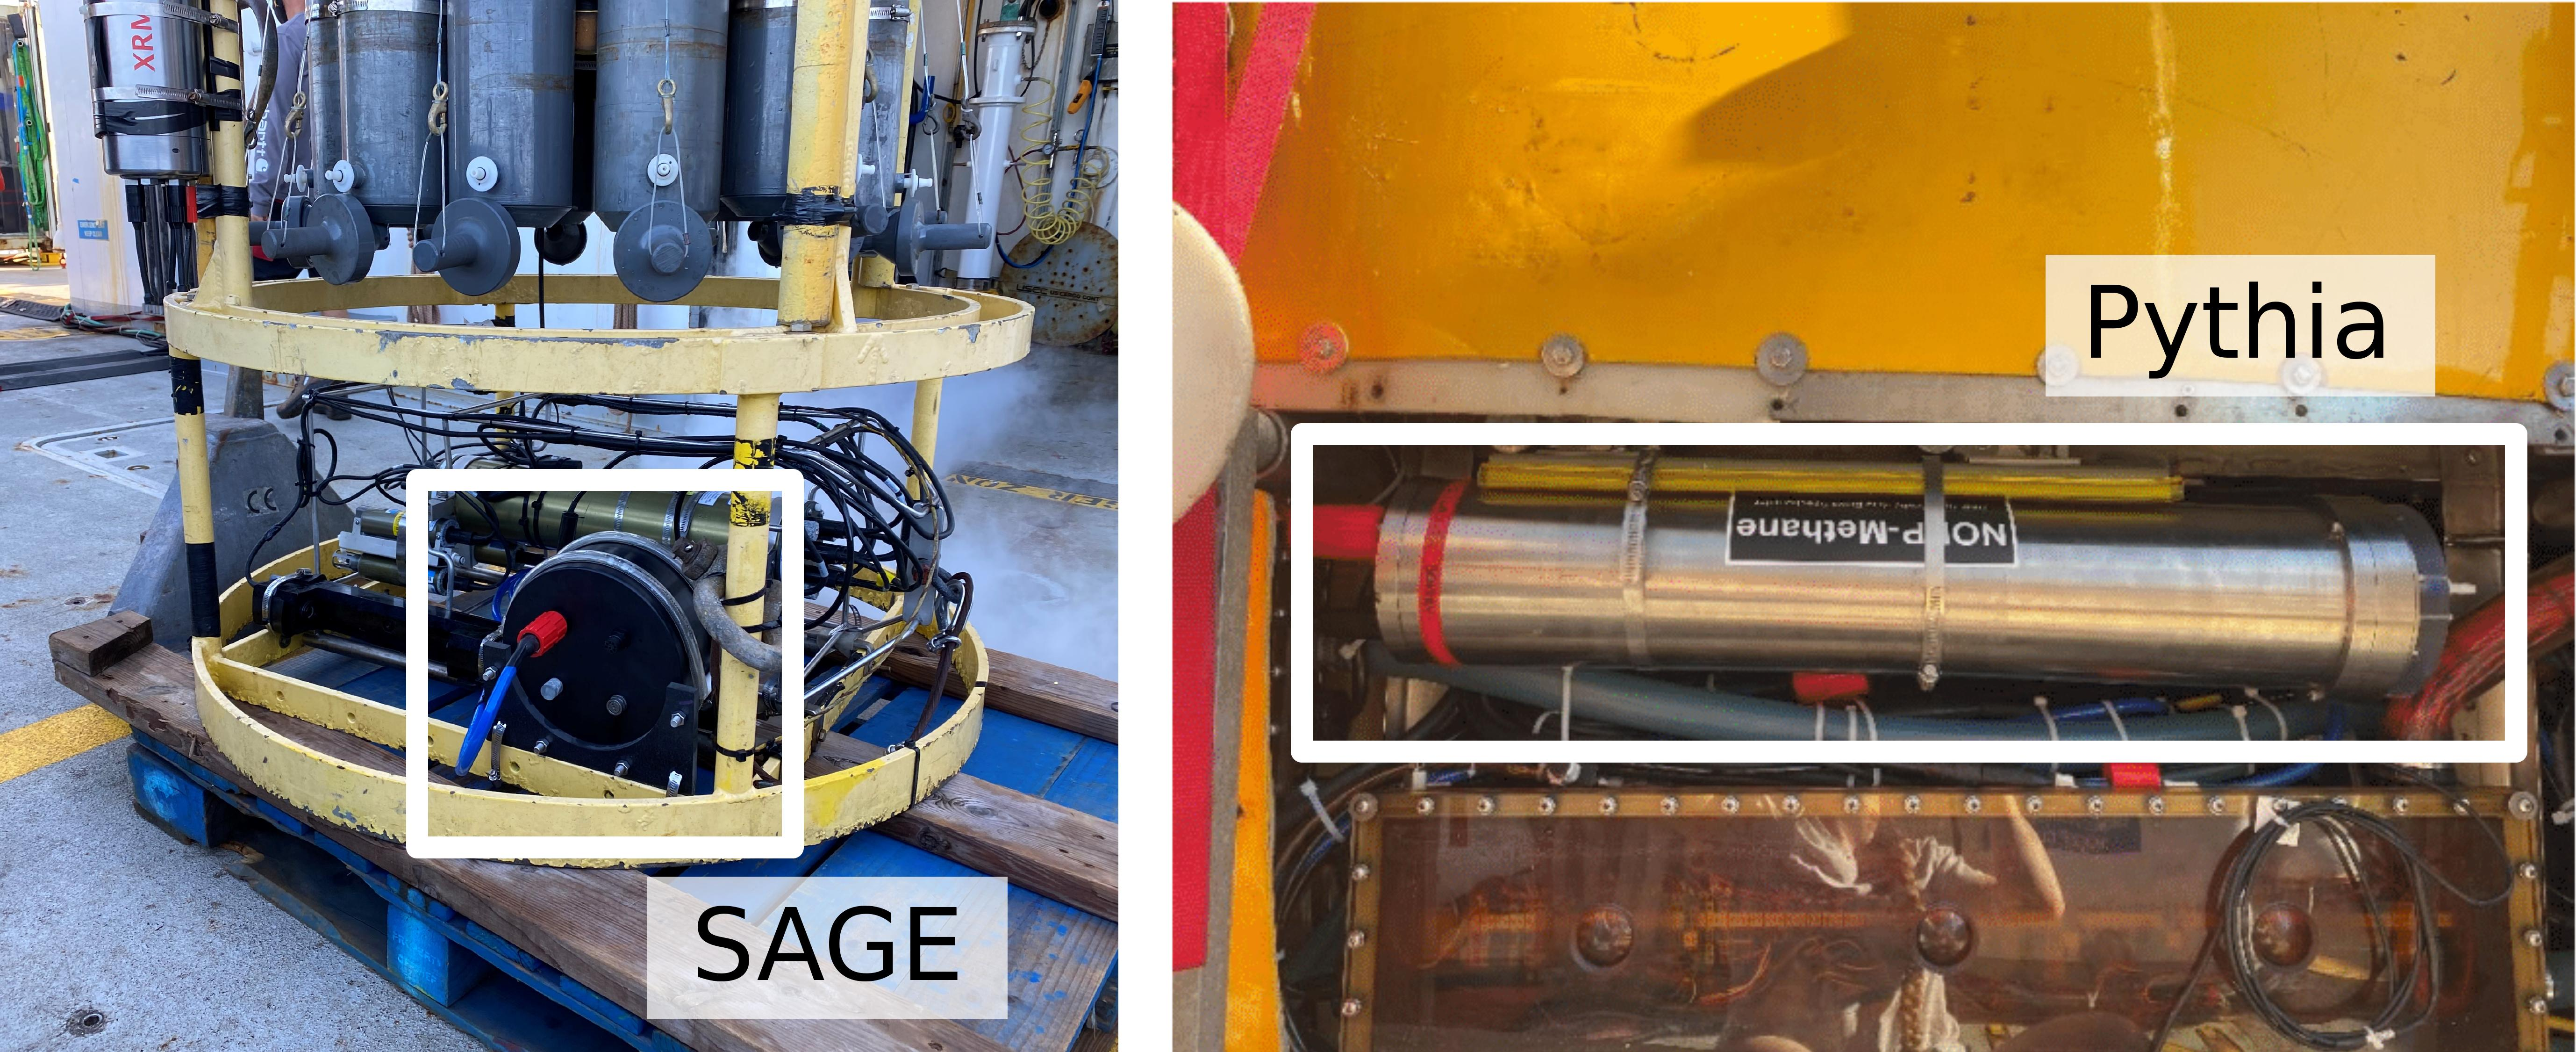
\includegraphics[width=\columnwidth]{figures/chap3_methane_sensor_mounting.jpg}
    \caption[Images of SAGE and Pythia methane instruments.]{\textbf{Images of the SAGE and Pythia methane instruments.} The SAGE and Pythia instruments were mounted on the rosette and AUV \emph{Sentry}, respectively.}
    \label{fig:sensor_mounting}
\end{figure}


\paragraph{SAGE}
\label{sec:sage}
SAGE is a dissolved gas sensing technology developed at the Woods Hole Oceanographic Institution (WHOI), and this expedition served as the first at-sea validation of the sensor's operation. SAGE technology has been previously described in \cite{kapit2021dissolved, kapit2021measurement}. Briefly, SAGE is based on infrared absorption spectroscopy performed on extracted gas from seawater via a gas permeable (and water impermeable) membrane. Once the gas enters the sensor, it fills a hollow-core optical fiber (HCF) which also guides light from a laser source tuned to measure the gas species of interest. The amount of target gas present is determined by measuring the amount of light absorption through the HCF using a photodetector. The prototype version of SAGE deployed on the research cruise was configured to measure methane in the range of 0-10,000 ppm. The resolution of the sensor was $<$1 ppm and the response time for the deployed configuration was approximately 12 minutes. For the scales of observations reported in this chapter (i.e., $<$2\% of the full scale of the observed signal), the instrument was minimally sensitive to temperature. SAGE is \SI{5.5}{\inch} long with a \SI{9}{\inch} outer diameter, and the power requirement was 7 W during this field deployment.

\paragraph{Pythia}
\label{sec:nopp}
Pythia is a novel deep-sea methane sensor developed utilizing real-time cavity ringdown spectroscopy (rt-CRDS) developed by WHOI~\autocite{michel2022gas} and Ring-IR Inc.~\autocite{Harb:12}, and capable of operating to \SI{4000}{\meter} depths. Pythia extracts dissolved gas from sea water using a large (\SI{113}{\centi\meter\squared}) surface area membrane. The extracted sample gas enters an optical cell where it is interrogated by a pulsed mid-infrared Quantum cascade laser (QCL). The laser light is absorbed by methane present in the cell, and the concentration of methane is determined by monitoring the pulsed ringdown signal from the cell using a mercury cadmium telluride (MCT) detector. While the response time of the sensor is slow, on the order of 35 minutes, the sensor is responsive to small ($<$2 ppm) changes in methane; the temperature sensitivity of Pythia has not yet been characterized. Pythia is ideally suited for long dives in environments in which changes to the methane concentration vary over long temporal and spatial scales. Details on the process for normalizing Pythia observations (which are strongly nonlinear and additionally require time correction) are provided in Appendix~\ref{app:perception:norm}. Pythia is \SI{24}{\inch} long with a \SI{4.5}{\inch} outer diameter, and was operated at a power range between 30-50 W during this field deployment.

\subsection{Analytical Procedure}
\label{sec:analytical}
Observations collected by sensors deployed on AUV \emph{Sentry}, including Pythia, were merged into a single dataframe using a common 1 Hz time reference; data were linearly interpolated onto this common time reference if they did not share an exact timestamp. With the exception of the derivative of ORP signal, all data for the purposes of visualization is smoothed using a centered rolling average over 5 minute intervals. Additionally, temperature, oxygen, and salinity measurements are normalized with respect to depth (as these quantities are anticipated to be functions of depth in the weakly stratified deep waters). Depth correction is performed by fitting a linear function to the average observation collected in \SI{20}{\meter} wide depth-bins, and computing the residuals of all data points with respect to this line (see Appendix~\ref{app:perception:depth} for plots of the linear functions). Rosette data is treated in the same fashion as \emph{Sentry} data. Down-cast and up-casts are removed from both \emph{Sentry} and rosette data streams for all visualizations.

\subsection{Transect Design and Execution}
AUV \emph{Sentry} and the rosette were deployed in the basin approximately \SI{16}{\kilo\meter} from the northern hydrothermal ridge structure, at (27.348152 N, 111.253108 W) with a course of \SI{295}{\degree} set to intersect the southern part of the ridge (Fig.~\ref{fig:bathy}). The \emph{Sentry} trackline was placed approximately 200-\SI{300}{\meter} north of the rosette to avoid any risk of entanglement. \emph{Sentry} was set in altitude hold mode, targeting \SI{120}{\meter} from the bottom (this places \emph{Sentry} at a depth of approximately 1750-\SI{1700}{\meter}, and at the top of its altitude-hold range). Rosette depth was targeted to be approximately 1650-\SI{1600}{\meter}, controlled primarily by the speed of the ship and length of the winch cable. These depths were designed based on an estimated model of the neutrally buoyant plume layer, as described in \cref{app:perception:model}. Leg 1 of the rosette trajectory was terminated at a planned stop at (27.393855 N, 111.364637 W), and Leg 2 was resumed at (27.460812 N, 111.527694 W); see Appendix~\ref{app:perception:niskin} for the schedule of bottle samples collected during Leg 2 presented in this manuscript. At the time of the transect, there were no known hydrothermal sites present over the sampling trajectory, save for the northern ridge. Hydrothermal vents in the southern basin were located approximately \SI{40}{\kilo\meter} further south from the transect starting location~\autocite{teske2016guaymas}.

\subsubsection{Modeling to Inform Transect Design}
\label{sec:afar_model}
The selection of heights for the rosette and AUV \emph{Sentry} was informed by a simple buoyancy model of expected plume characteristics on the ridge, and known operational constraints of AUV \emph{Sentry} (i.e., an absolute floor and ceiling of operation above the bottom). Using an adapted plume crossflow model developed by~\cite{tohidi2016highly} (see Appendix~\ref{app:perception:model} for more detailed information) with a nominal current crossflow value of \SI{0.1}{\meter\per\second}, vent temperature of \SI{340}{\celsius}, and estimated background seawater stratification as per~\cite{speer1989model}, a neutrally-buoyant layer was estimated to form between \SI{1570}{\meter} and \SI{1750}{\meter}. The depths for the rosette (1600-1650 m) and AUV \emph{Sentry} (1700-1750 m) were set given this information in order to target both the upper and lower estimated neutrally buoyant layer (NBL), respectively. The NBL was targeted to increase the likelihood of intersecting plume waters during the transect over a broad, multi-kilometer scope. This is in contrast with targeting the plume buoyant stem, which though significantly easier to distinguish from background seawater, may only have an expression on the order of several square meters.

\subsubsection{Real-Time Data Feedback and Watchstanding}
During the transect, data from the standard rosette sensors were available in near-real time at the watchstander station in the shipboard computer lab. This allowed watchstanders to monitor the depth of the rosette and relay requests to the winch operator on deck, and display the data on live-updating visualizers. AUV \emph{Sentry} relayed occasional data packets up to 128 bytes in length at a rate of approximately 0.01 Hz. These data packets were subsequently graphed on a computer monitor that was linked to the \emph{Sentry} network. A total of 600 messages with information about the standard science instruments on \emph{Sentry}, and 583 messages with information from the Pythia instrument were transferred during the transect.

\section{Results}
\label{sec:afar_results}

% Methane Instruments
\subsection{Methane Measured by Spectroscopic Instruments}
\label{sec:methane_results}
Elevated methane was observed over a spatial scale of several kilometers, significantly rising as both AUV \emph{Sentry} and the rosette approached the source of known hydrothermalism on the transect (Fig.~\ref{fig:methane_distance}). As both methane instruments used on this cruise were in active development, methane observations are reported as normalized values from 0 to 1. A normalized value of 0.5 is used as a conservative threshold for classifying elevated methane measurements. Pythia, mounted on \emph{Sentry}, reached and exceeded this threshold for elevated methane starting at approximately \SI{3}{\kilo\meter} from the hydrothermal reference point at (27.407489 N, 111.389893 W); SAGE, flying nearly \SI{50}{\meter} higher in the water column, reached this threshold starting \SI{1.5}{\kilo\meter} away. For a less conservative threshold of 0.3, these spatial detection points are reached 6.8 km and 2.2 km away, respectively. SAGE observed a sharp peak of methane just under \SI{1}{\kilo\meter} from the reference source, with rapid decline of observable methane soon after. In contrast, Pythia reached a methane peak essentially at the \SI{0}{\kilo\meter} reference point, and shows a gradual decline in methane as \emph{Sentry} descends into a graben just north of the hydrothermal ridge; the rosette was pulled from the water at the ridge. The difference in spatial detection patterns indicated by these instruments may be a function of the different sensor modalities/sensitivities, the natural structure of the neutrally-buoyant layer, and the relative position of the two platforms within it. 

\begin{figure}[h!]
    \centering
    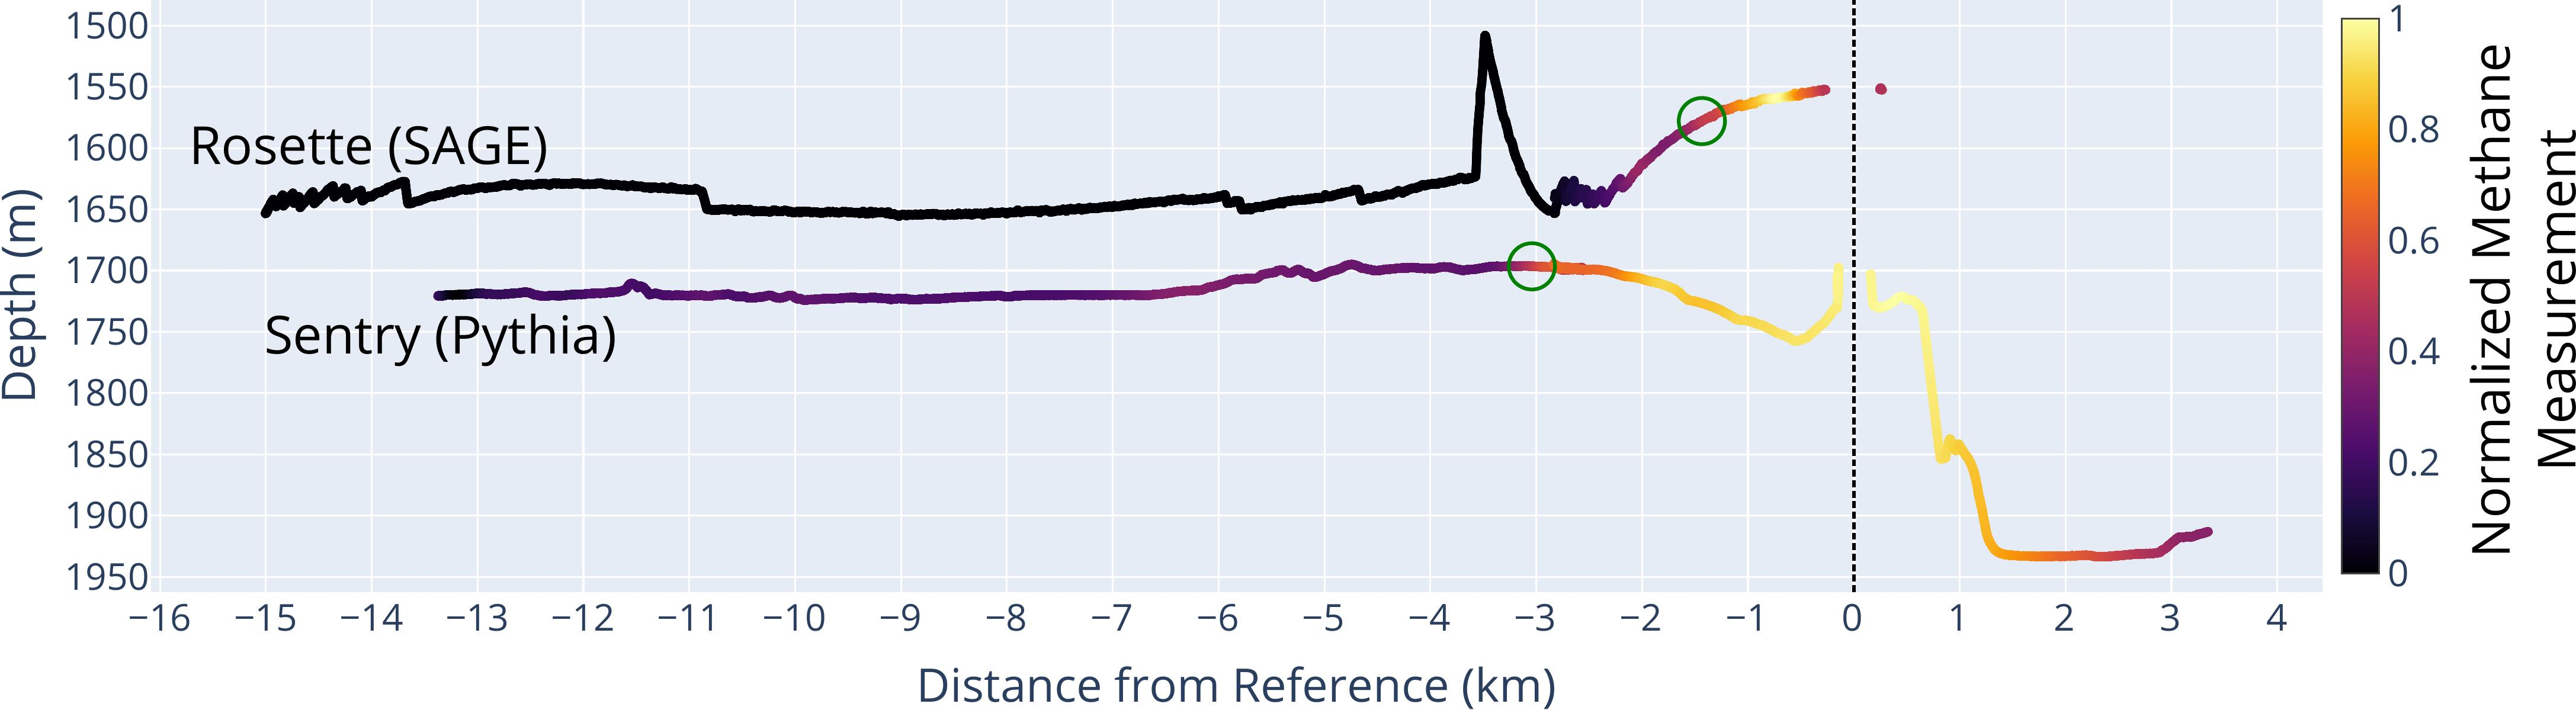
\includegraphics[width=1\columnwidth]{figures/chap3_methane_over_distance.jpg}
    \caption[Methane observations collected over the transect.]{\textbf{Methane observations collected over the transect.} Normalized methane values observed with both SAGE (rosette) and Pythia (\emph{Sentry}) over reference distance from (27.407489 N, 111.389893 W). The transect begins at the left of the plot and proceeds to the right. Strong methane anomalies, defined as points above a conservative threshold of 0.5 normalized values, are present starting \SI{3}{\kilo\meter} from the reference source as observed by Pythia, and \SI{1.5}{\kilo\meter} as observed by SAGE (open green circles).}
    \label{fig:methane_distance}
\end{figure}


% Methane + Ammonium
\subsection{Methane and Ammonium Measured with the Rosette}
Ammonium is a microbial energy source and reduced compound that is produced by the hydrothermal vents at Guaymas Basin. It is expected that ammonium and methane behavior in the basin will behave similarly, providing a ``check'' on the methane trends observed in methane bottle samples, and recorded by SAGE. Focusing primarily on Leg 2 of the rosette transect, there is a correspondence between methane and ammonium elevation in the approach to the hydrothermal ridge (Fig.~\ref{fig:bottles}). Methane samples processed directly from Niskin bottles as outlined in Sec.~\ref{sec:bottles} show a peak methane concentration of 3000-4000 nM (this range is associated with the extremes of calibrated extraction efficiencies valid for the equipment used), approximately \SI{0.75}{\kilo\meter} from the hydrothermal reference point. Ammonium tracks closely with methane, at 3-4 times smaller concentration, reaching a peak of approximately 1000 nM. 

Normalized methane observations by SAGE generally follow the trends shown by the bottle samples, similarly showing a spatial peak at \SI{0.75}{\kilo\meter}. However, by its nature, SAGE yields a significantly more resolved signal; a small, secondary peak is observed by SAGE at \SI{2}{\kilo\meter} from the reference point which is essentially missed by the bottle samples. Additionally, by virtue of operating continuously, there is no need for human interaction (unlike for processing bottle samples, which can require time-intensive \emph{ex situ} analysis). 

\begin{figure}[h!]
    \centering
    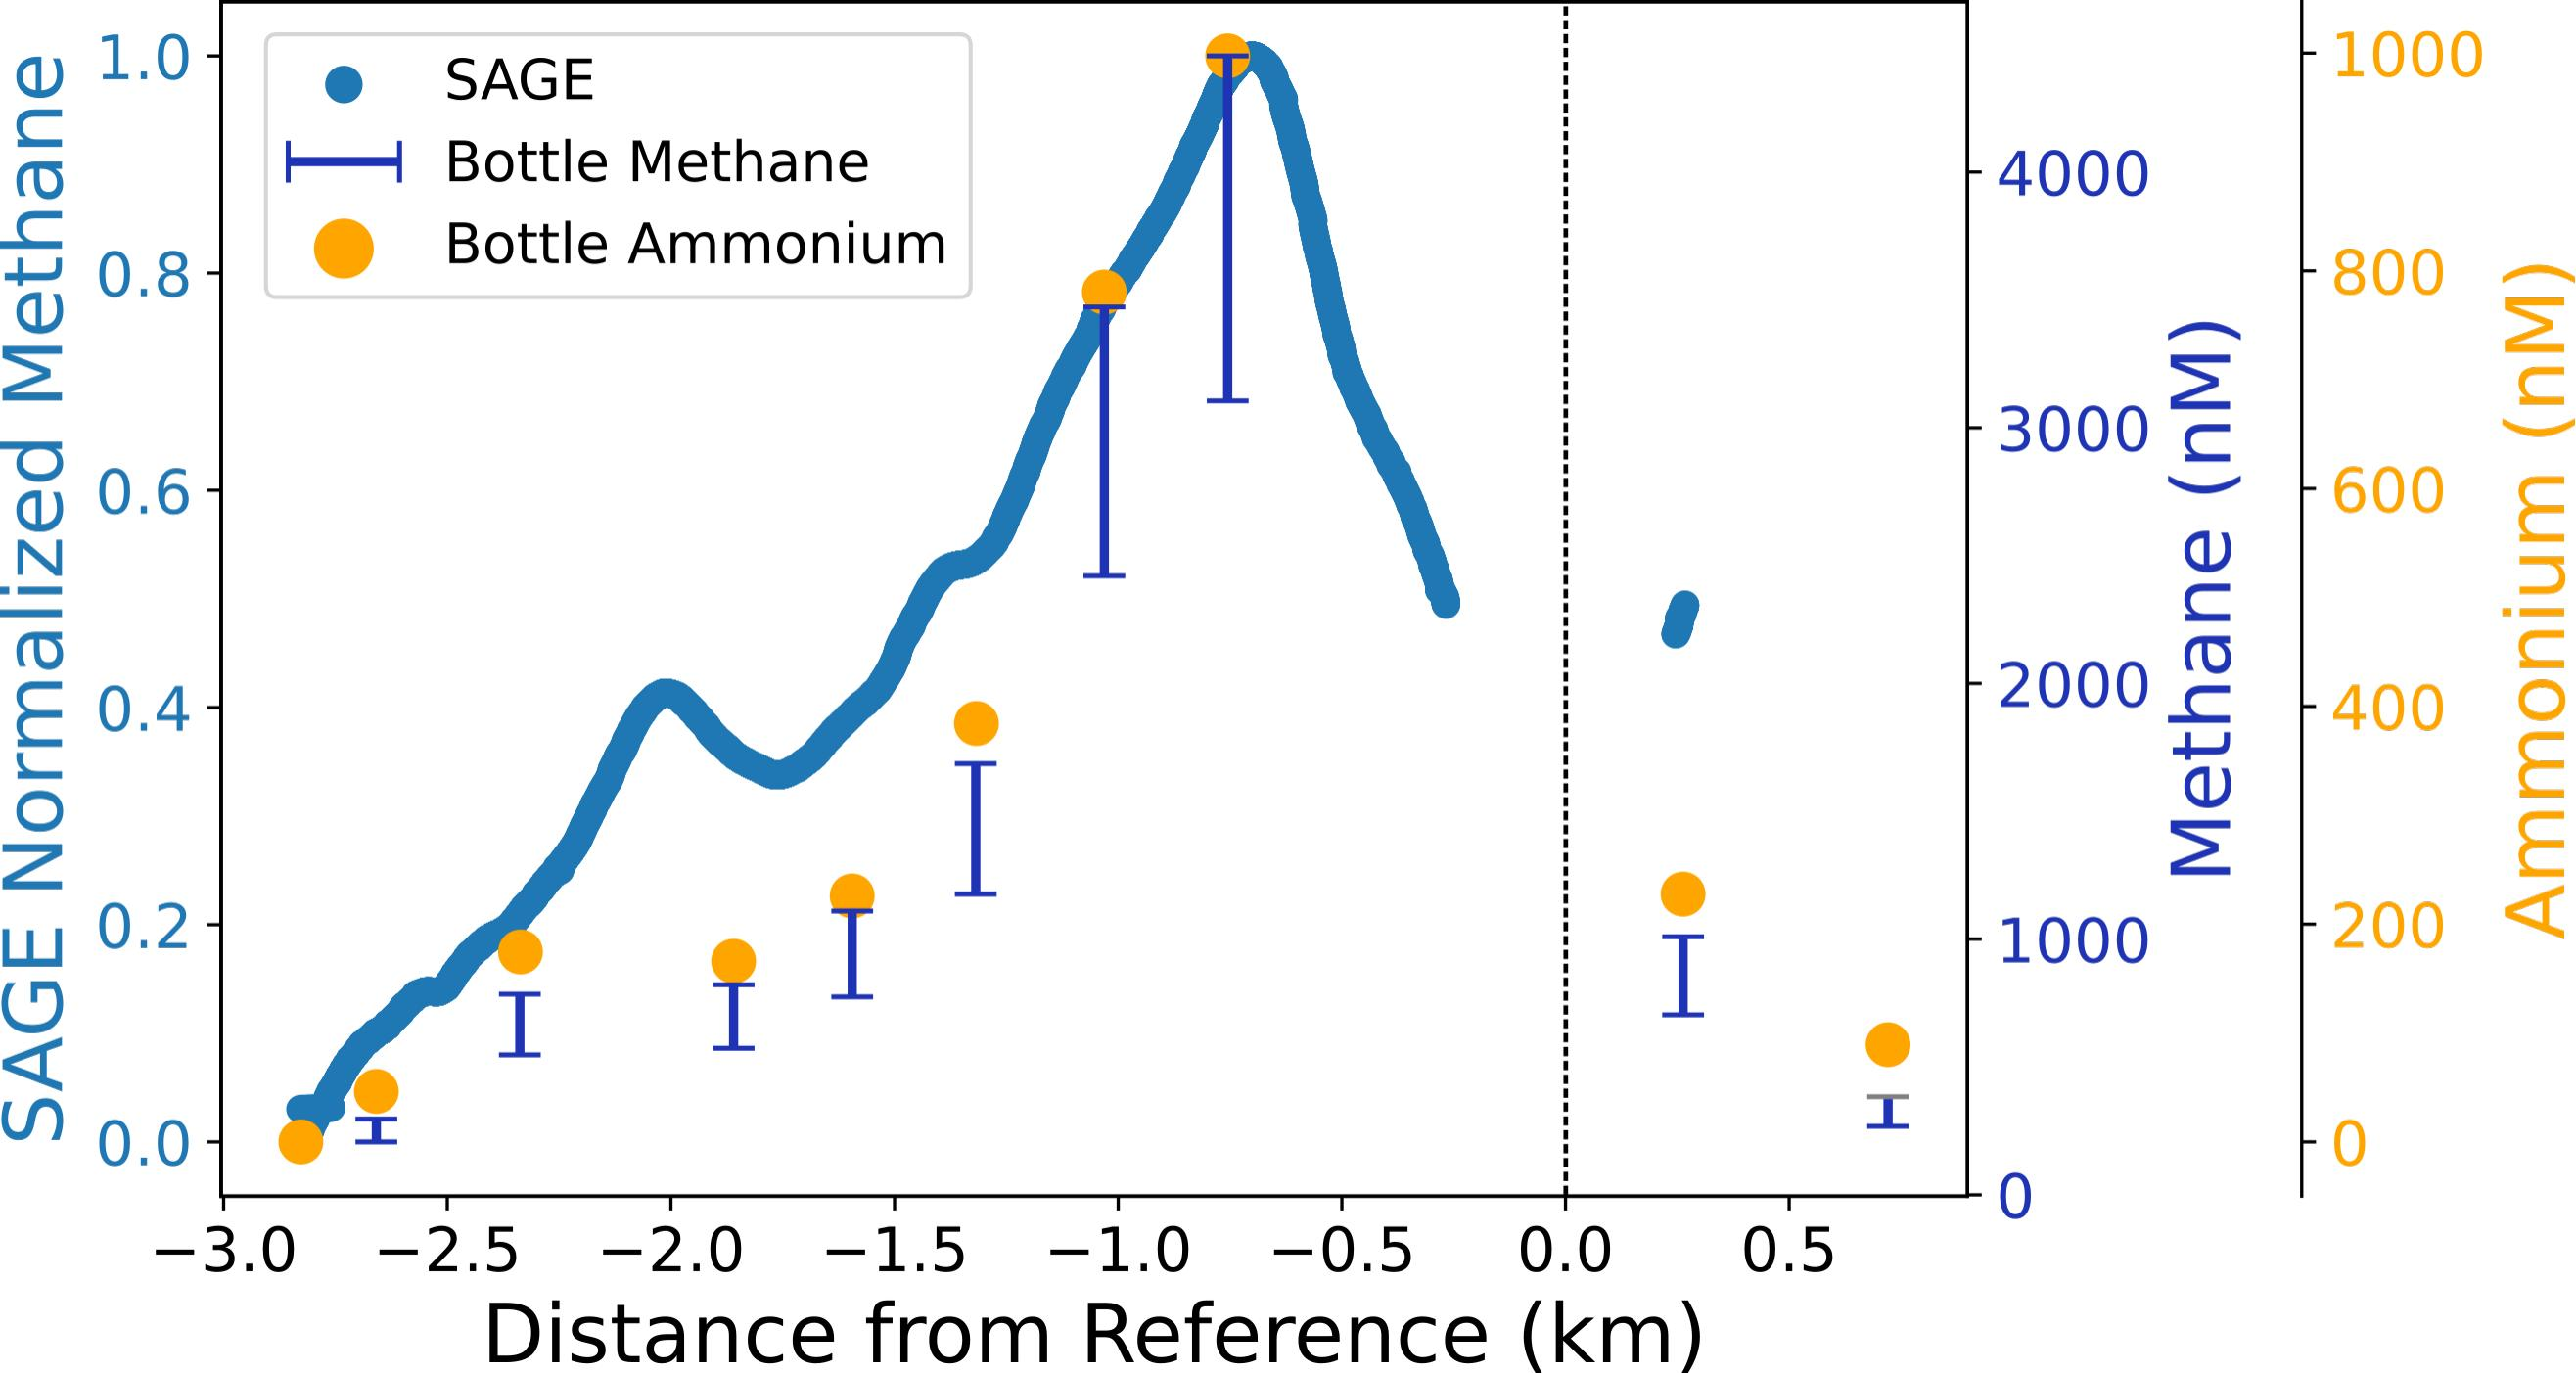
\includegraphics[width=\columnwidth]{figures/chap3_bottle_norm.jpg}
    \caption[Methane observations compared to ammonium concentrations.]{\textbf{Methane observations compared to ammonium concentrations.} Normalized methane measurements by SAGE plotted with methane measurements taken from Niskin bottle samples (as measured by DGEU/GGA equipment) and ammonium measurements. Bottle methane measurements are reported as a range to reflect sensitivity of the measurement procedure to a calibrated extraction efficiency. All measurements trend towards a peak observation of methane and ammonium \SI{0.75}{\kilo\meter} from the reference source. SAGE additionally observes a secondary peak approximately \SI{2}{\kilo\meter} from the source, which is essentially missed by the bottle sample schedule.}
    \label{fig:bottles}
\end{figure}


% Turbidity
\subsection{Turbidity}
\label{sec:turbidity_results}
Turbidity is a commonly used indicator for detecting hydrothermalism from smoking vents; particulate matter produced by smoking vents can remain suspended in the neutrally buoyant layer, acting as a non-conservative tracer for hydrothermalism~\autocite{feely1992tracking}. In the Guaymas Basin, suspended particulates have been shown to be composed of metals like iron, aluminum, and manganese~\autocite{scholz2019shelf} and are primarily mixed into bottom waters from hydrothermal activity. Here, turbidity measurements are reported as normalized values to make direct comparison between the platforms straightforward; in absolute terms, the transmissometer on the rosette reported beam attenuation values between 0-0.2 and the OBS on \emph{Sentry} observed backscatter values between 0.08-0.14. The OBS on \emph{Sentry} encountered an error from the beginning of the dive, potentially caused by a persistent air bubble, until approximately \SI{4.5}{\kilo\meter} from the the ridge reference point; these early measurements are omitted. 

Elevated turbidity (defined by a conservative threshold of 0.5 in the normalized data) was observed with the transmissometer on the rosette starting approximately \SI{2.2}{\kilo\meter} from the reference source and \SI{3.3}{\kilo\meter} with the OBS on \emph{Sentry} (Fig.~\ref{fig:turbidity_distance}). Even with a less conservative threshold (0.3) these detection points only slightly improve to 2.5 km and 3.4 km respectively. With \emph{Sentry}, a rapid decline in turbidity within tens of meters west of the source reference (positive distance in Fig.~\ref{fig:turbidity_distance}) is observed. This may be indicative of the direction of prevailing crossflow (southeast) in the basin, which would directionally bend a buoyant plume stem and advect the neutrally buoyant layer.

\begin{figure}[h!]
    \centering
    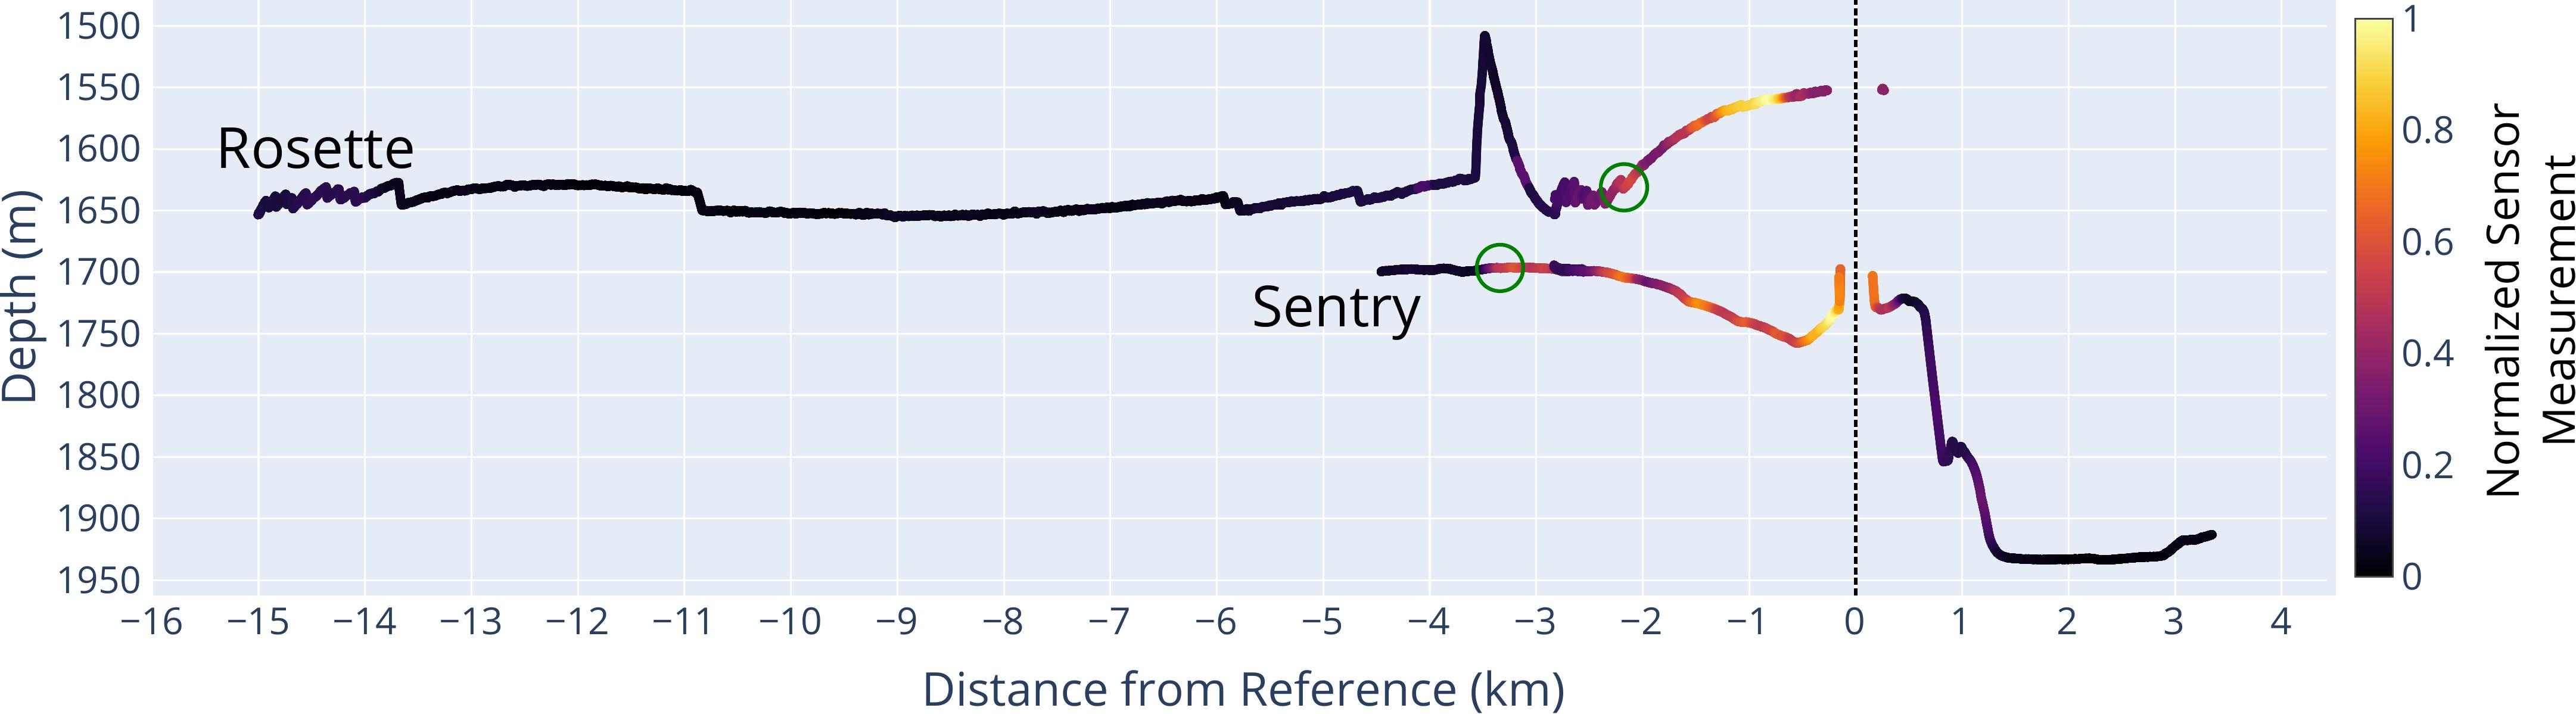
\includegraphics[width=\columnwidth]{figures/chap3_turbidity_over_distance.jpg}
    \caption[Turbidity measurements collected during transect.]{\textbf{Turbidity measurements collected during the transect.} Turbidity observed as beam attenuation on the rosette transmissometer and optical backscatter on AUV \emph{Sentry} instruments. \emph{Sentry} encountered a sensor error until approximately \SI{4.5}{\kilo\meter} from the ridge reference point. After this point, elevated turbidity is detectable throughout the dive, with significant elevations within \SI{3.3}{\kilo\meter} east of the ridge reference point, dissipating within tens of meters to the west. Elevated turbidity is observed by the rosette \SI{2.2}{\kilo\meter} from the ridge reference point to the east.}
    \label{fig:turbidity_distance}
\end{figure}


% ORP
\subsection{Oxidation Reduction Potential}
AUV \emph{Sentry} carries an ORP sensor; there was no comparable sensor on the rosette. ORP sensors are commonly used in hydrothermal plume hunting, and can be a strong indicator of recently emitted hydrothermal fluids. The derivative of ORP (noted here as dORPdt) is particularly used, in which negative dORPdt values typically indicate transition from background water into hydrothermal fluid. During the transect, only one significant dORPdt deviation was observed, within \SI{200}{\meter} from the ridge reference point (Fig.~\ref{fig:orp_distance}). 

\begin{figure}[t!]
    \centering
    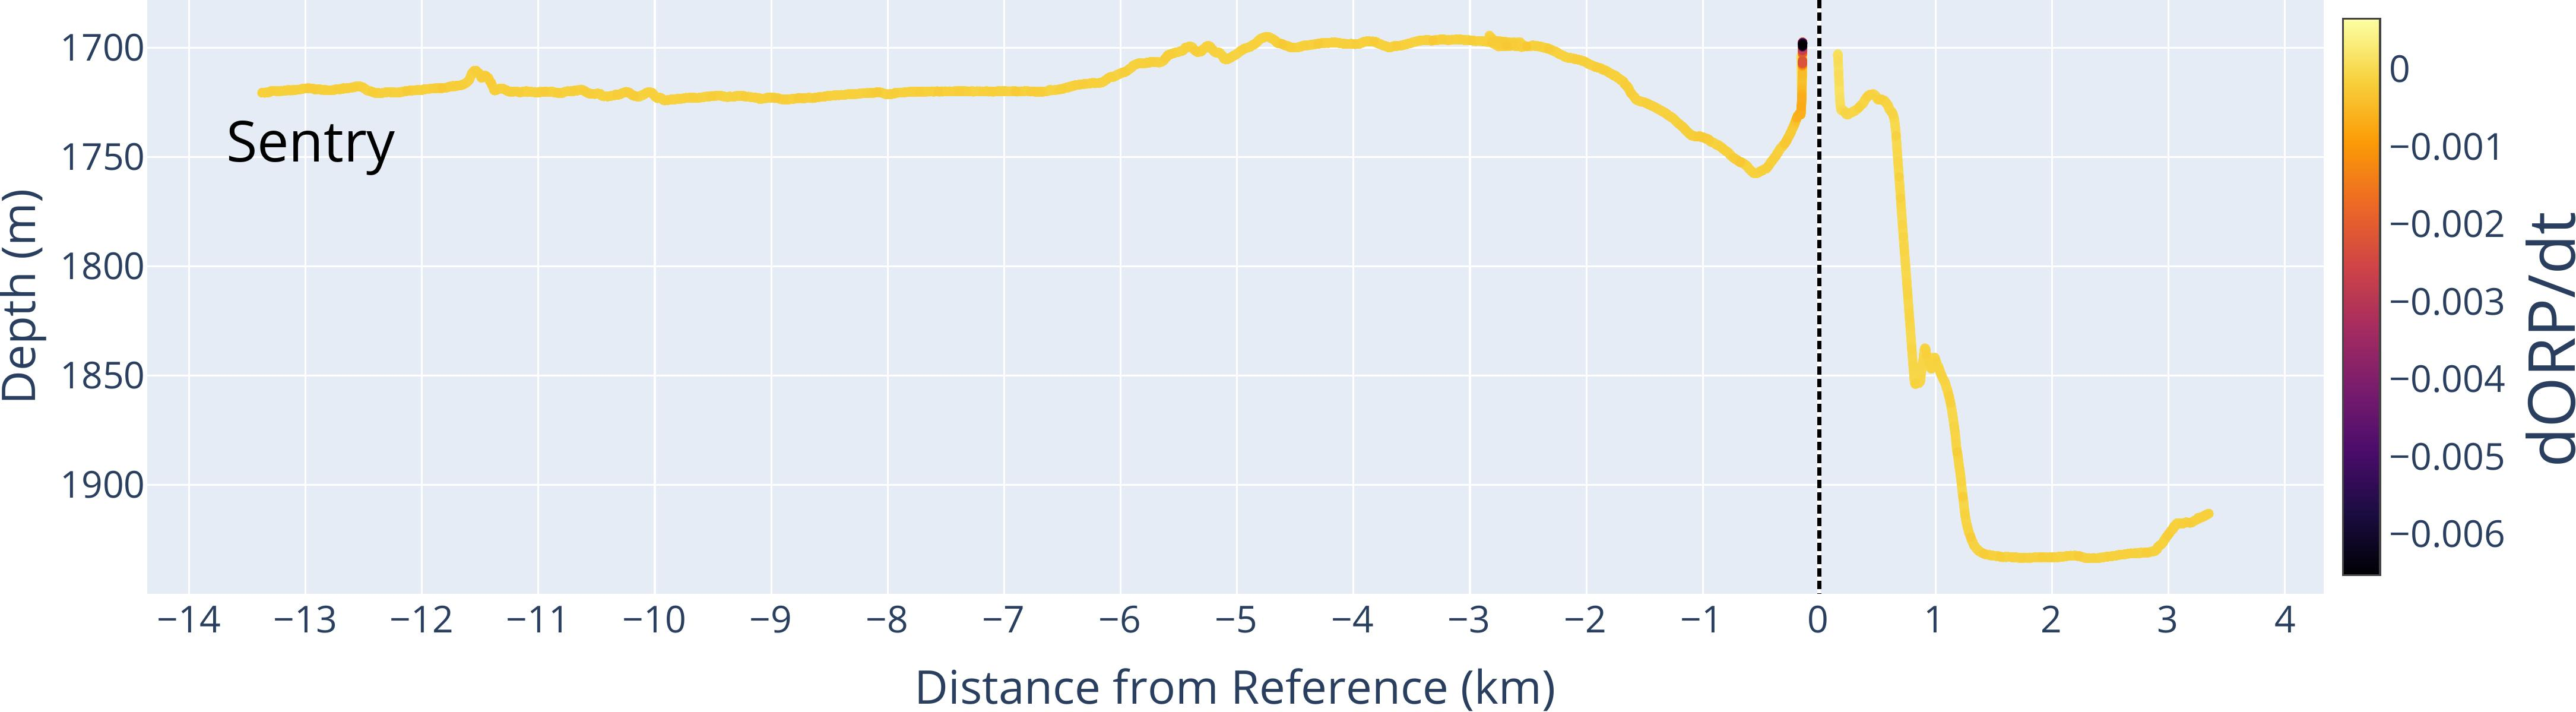
\includegraphics[width=\columnwidth]{figures/chap3_orp_over_distance.jpg}
    \caption[Oxidation-reduction potential measurements collected during transect.]{\textbf{Oxidation-reduction potential measurements collected during transect.} The derivative of ORP observed by data collected on AUV \emph{Sentry}. Negative slopes are indicative of entering hydrothermal fluids. Only one region of the transect demonstrated a significant reaction to ORP, within \SI{200}{\meter} of the reference point.}
    \label{fig:orp_distance}
\end{figure}

% Temp, Salt, O2
\subsection{Temperature, Salinity, and Oxygen}
\label{sec:o2_temp_salt}
Temperature, salinity, and oxygen are expected to be weakly stratified in deep ocean waters, however fluids from hydrothermalism should register as anomalies when present. The magnitude of valid anomalies (i.e., anomalies that positively identify fluids impacted by hydrothermalism) can be exceedingly small; temperature at a vent can be hundreds of degrees Celsius, but anomalies in the water column on the spatial order of only \SI{10}{\meter} can be measured as single degrees, and within a neutrally-buoyant plume on the order of hundreds of meters from the source, only register a few hundredths of a degree~\autocite{yoerger2007autonomous}. 

Temperature, salinity, and oxygen anomalies are computed according to the process described in Sec.~\ref{sec:analytical} and the results are shown in Fig.~\ref{fig:o2_temp_salt}. Salinity anomalies, although apparently coherent, are reported within the empirical sensor noise for the CTD instruments on both the rosette and \emph{Sentry}. Temperature anomalies on the scale of hundredths of a degree are observed throughout the transect, with two key regions of high temperature anomaly, one located 6-12 km from the reference source, and the other within 3 km of the source. Both the rosette and \emph{Sentry} observe these regions; with \emph{Sentry} observing the first anomaly in a narrower margin between 8-11 km from the reference source. The first region of positive temperature anomaly closely corresponds with marginally fresher water; whereas the region of higher temperature anomaly near the source is not consistently matched in salinity (the rosette observes more salinity content, whereas \emph{Sentry} observes neutral or slightly less salinity content). Oxygen is reported as nominal or slightly depleted within the regions of notable temperature and salinity anomaly.

\begin{figure}[h!]
    \centering
    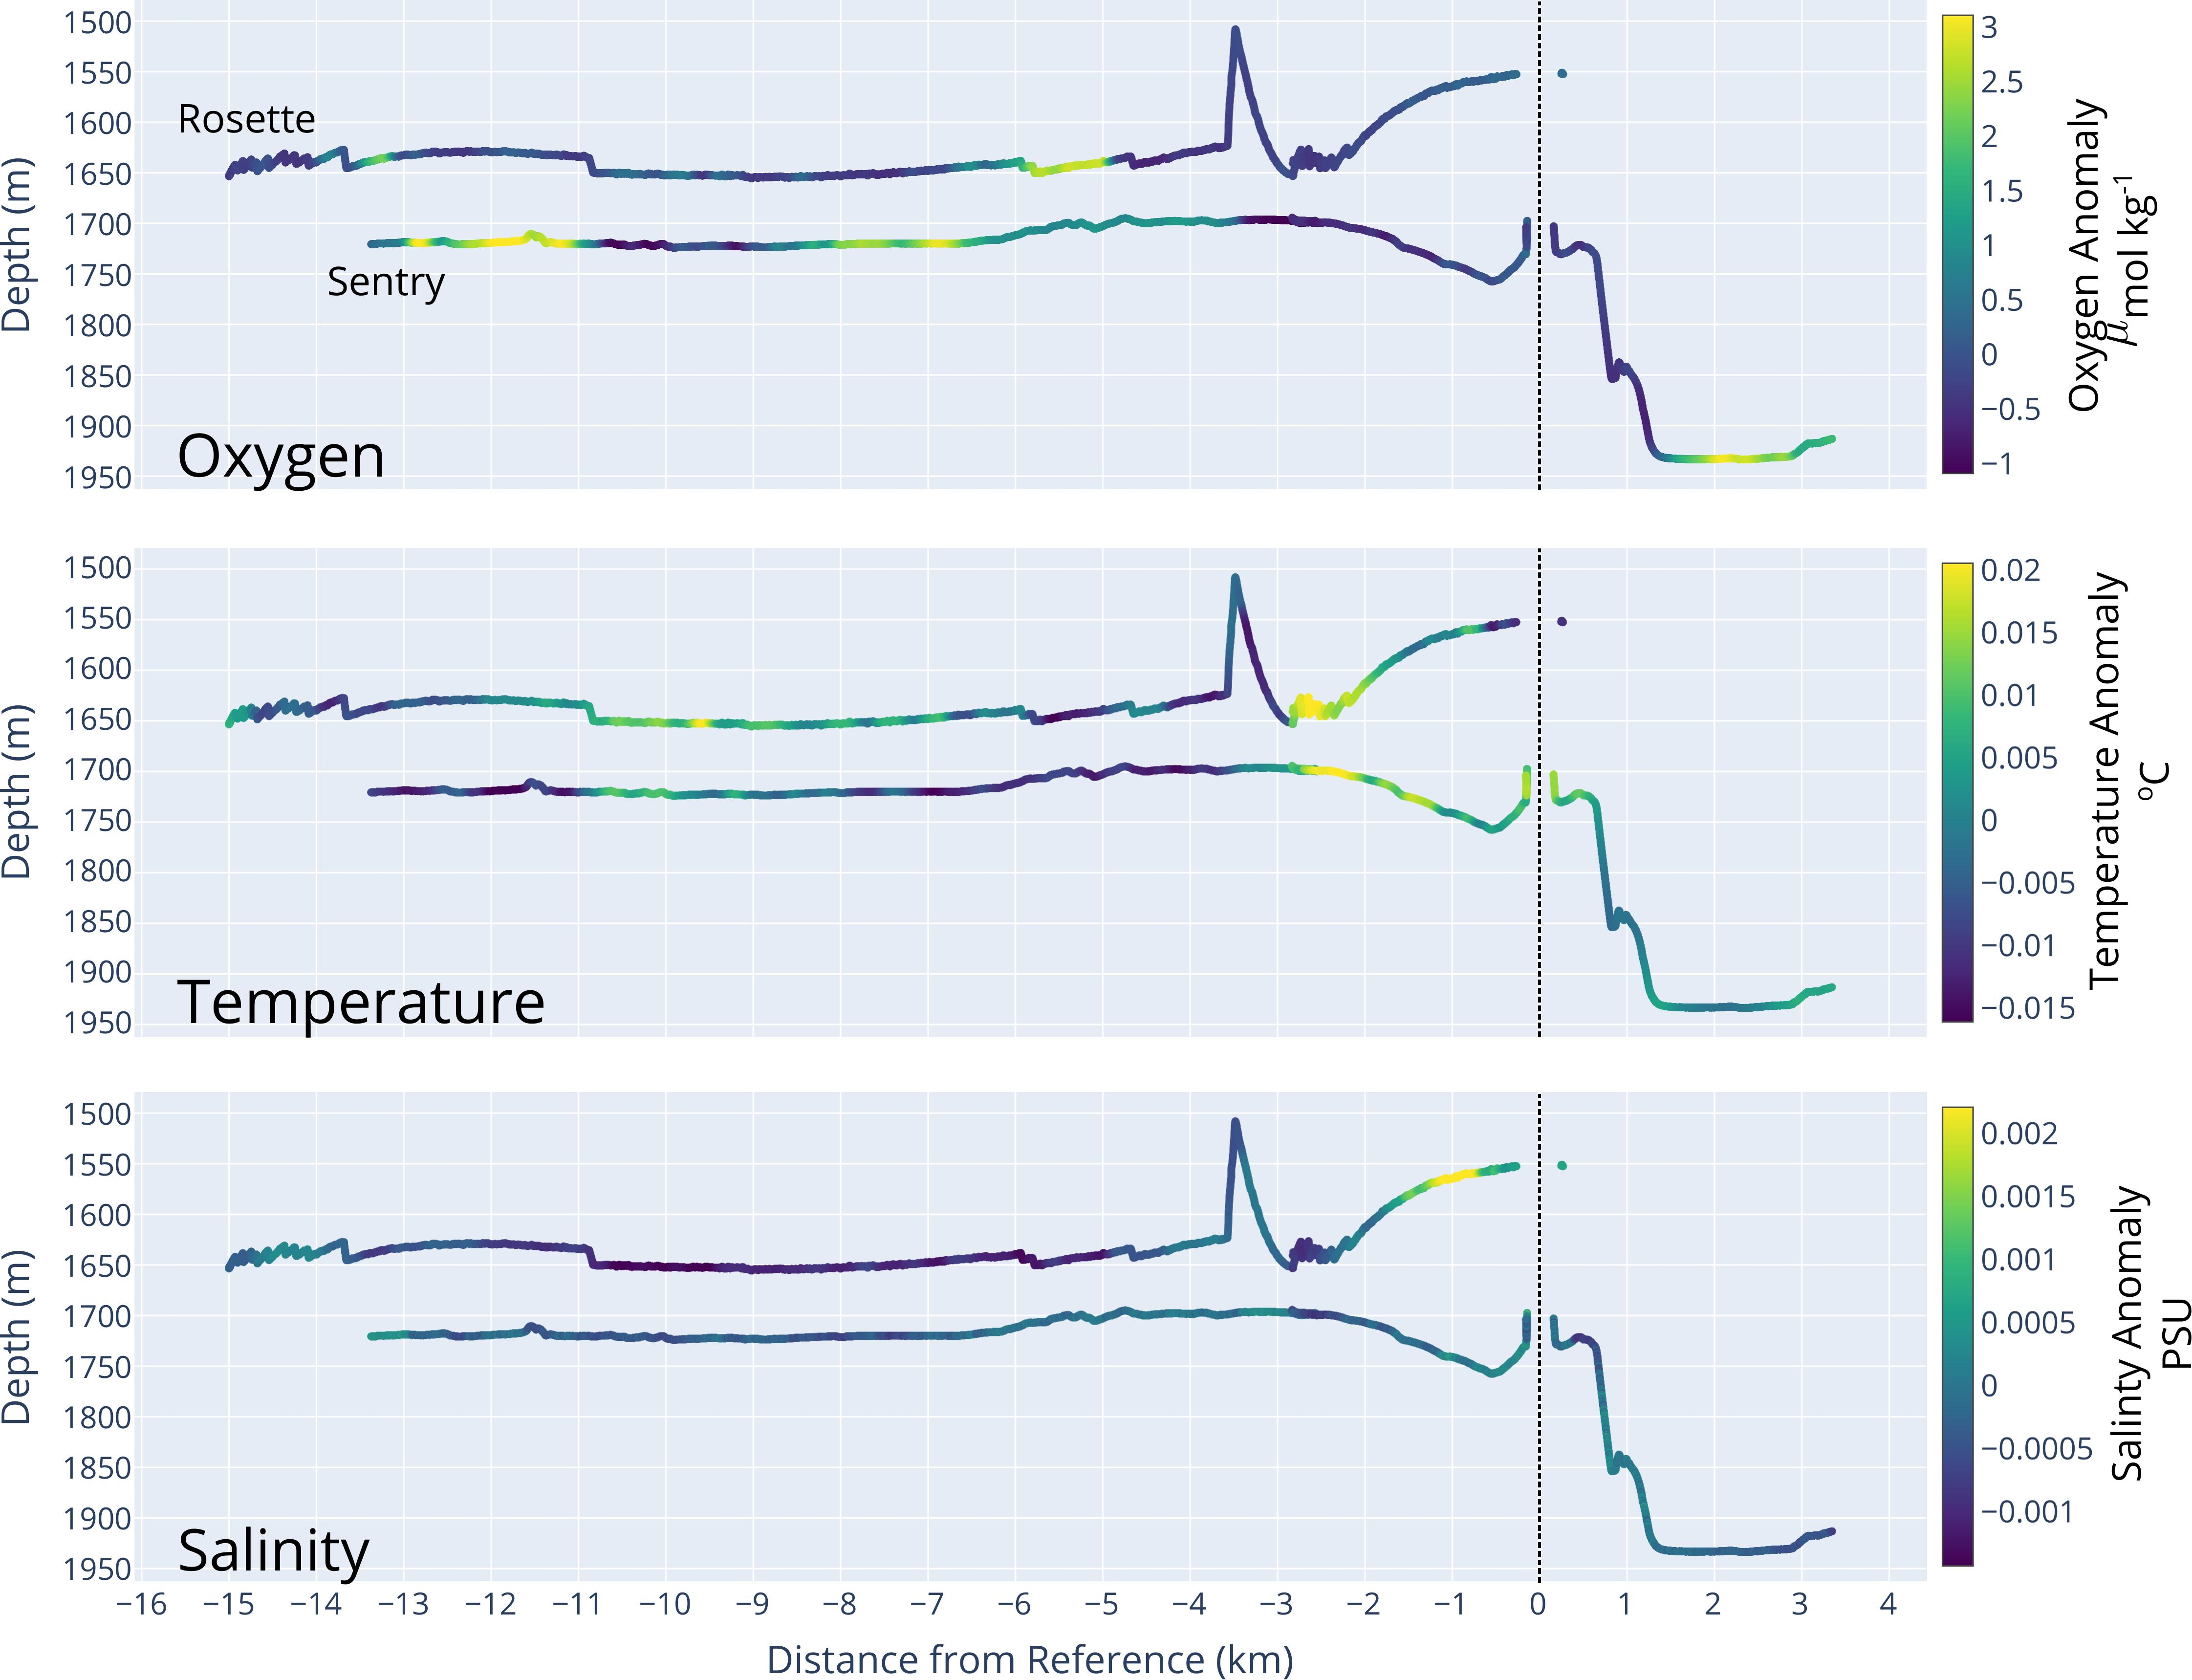
\includegraphics[width=1\columnwidth]{figures/chap3_o2_temp_salt_over_distance.jpg}
    \caption[Depth-corrected oxygen, temperature, and salinity measurements collected during transect.]{\textbf{Depth-corrected oxygen, temperature, and salinity over reference distance.} Two notable regions of high temperature deviation from expected temperature are observed between 6-12 km (rosette; 8-11 km by \emph{Sentry}) and within 3 km of the reference source. The first region of temperature anomaly is closely matched with fresher salinity measurements; whereas salinity is measured as marginally higher near the reference source by the rosette CTD and nominal or lower by the \emph{Sentry} CTD. In both regions, oxygen is nominal or slightly depleted, with regions of notably elevated oxygen at the boundary of these regions.}
    \label{fig:o2_temp_salt}
\end{figure}

The first region of interest, far afield from the plume reference point, appears coherent and has similar detection qualities to the near-reference region; however, given the typical expectation of temperature dissipation from hydrothermal sources, it would be surprising if this first region were connected with hydrothermalism. The shape of the warm, slightly fresher and oxygen depleted intrusion (laterally broad higher in the water column, and appearing to narrow based on the observations taken by the rosette and \emph{Sentry} approximately 50 m offset in altitude) also does not follow expected patterns in a neutrally buoyant plume layer. Lack of significant methane and turbidity observations in this same region, as presented in Sec.~\ref{sec:methane_results} and Sec.~\ref{sec:turbidity_results} respectively, additionally casts doubt on hydrothermalism as a driver for this anomaly. Water mass mixing between the bottom waters, largely sourced from Pacific Deep Waters and the Pacific Intermediate Waters~\autocite{bray1988water} may be an alternative explanation, but is out of scope for this study to investigate. 


\section{Discussion}

\subsection{Sensor Cross-Correlations}
\label{sec:correl}
Successfully detecting hydrothermalism in the deep ocean is a significant challenge, and detection may be most effective using a combination and corroboration of anomalies across multiple sensor inputs~\autocite{jakuba2007stochastic}. Here, the cross-correlation between sensors mounted on each of the platforms is investigated. Both a global and rolling Pearson correlation coefficient were computed, showing overall correlation trends and situation dependent correlation, respectively.

Fig.~\ref{fig:global_corr} shows the global correlation among sensors mounted on the rosette individually over Leg 1 and Leg 2, in addition to sensors mounted on \emph{Sentry}. In the absence of significant geochemical features in a target environment, it is expected that no or only weak correlation will be computed globally, as individual sensor noise (which is independent) will dominate the computation; when geochemical structure is present in the environment, it is expected that weak to strong global correlation will be computed as the environment is imposing a (shared) signal across at least a subset of sensors. This is well illustrated by the cross-correlation matrices for the rosette legs, with global coefficients for Leg 1 reporting no correlation between sensors save for a slightly negative correlation between temperature and oxygen, and for Leg 2 reporting weak to strong correlations between all sensors, with notably strong positive correlation between turbidity and methane. Interestingly, in Leg 2 a negative correlation is reported between temperature and methane, and a positive correlation is measured between methane and oxygen measurements. This runs directly counter to expectations; and also counter with the relationships observed by \emph{Sentry} which marks relationships between methane and temperature as positively correlated, and between methane and oxygen as negatively correlated. 

\begin{figure}[h!]
    \centering
    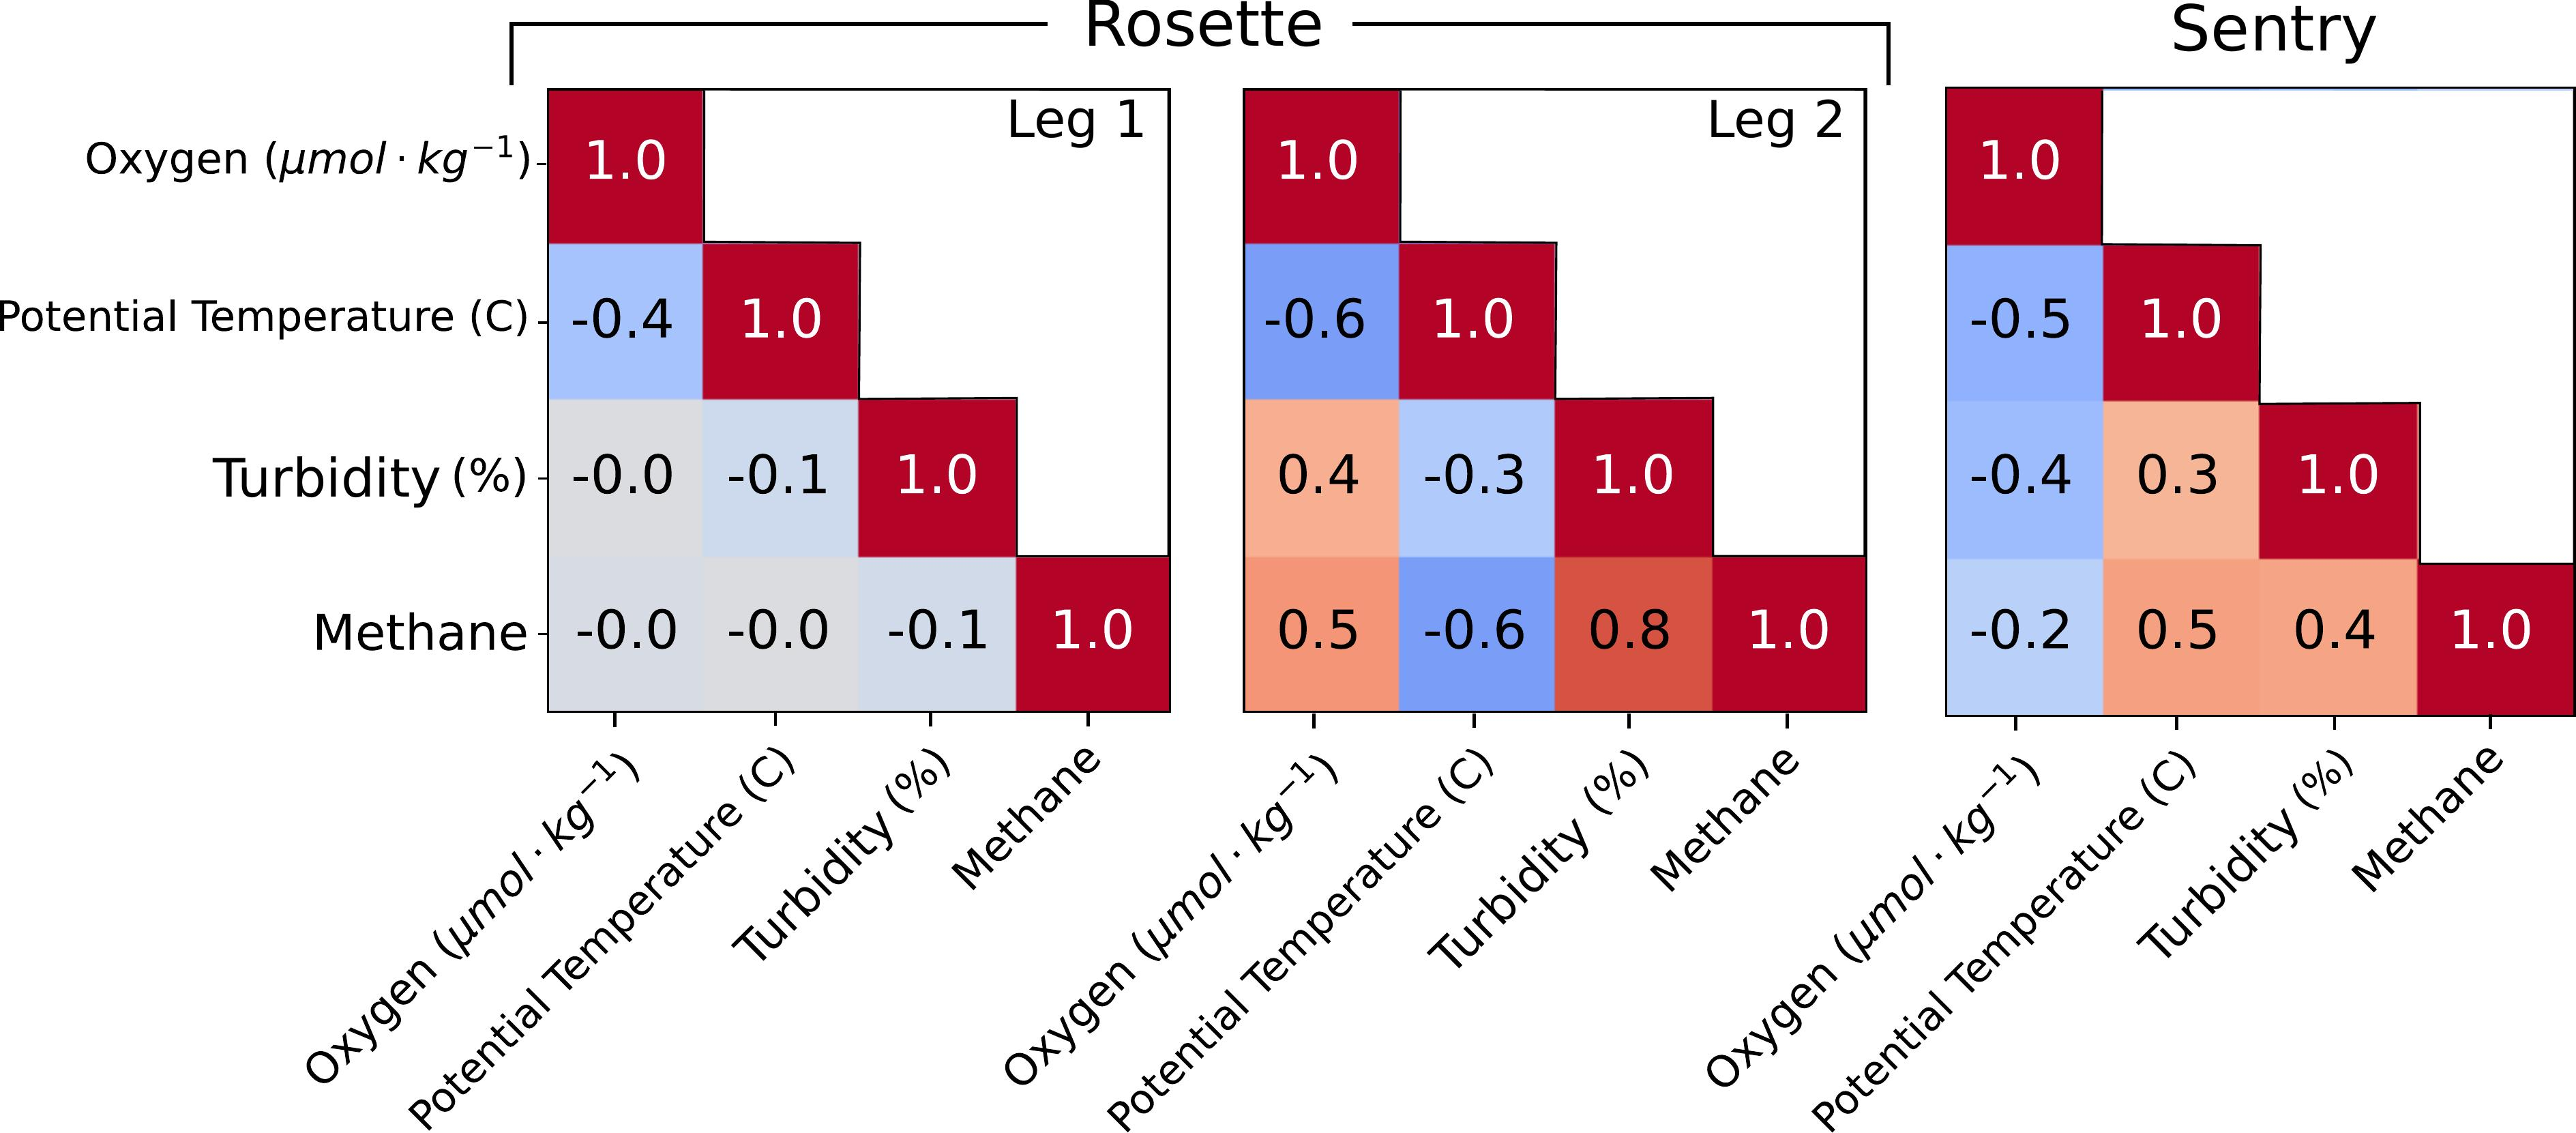
\includegraphics[width=0.9\columnwidth]{figures/chap3_all_global_corr.jpg}
    \caption[Global Pearson correlation coefficients between sensors mounted on the rosette and \Sentry.]{\textbf{Global Pearson correlation coefficient between sensors mounted on the rosette and \emph{Sentry}.} Correlation differences between Leg 1 (far from the reference point) and Leg 2 (near the reference point) are indicative of different sensor correlation behaviors with respect to ambient seawater conditions and hydrothermal fluid interception. \emph{Sentry} correlation coefficients reflect an expected relationship between temperature and methane (positive), methane and oxygen (negative), and turbidity and methane (positive) that may be stereotypically associated with hydrothermal fluids. In contrast, the Leg 2 rosette correlation factors do not meet this expectation, despite showing strong overall correlative structure.}
    \label{fig:global_corr}
\end{figure}

The difference between correlative behaviors between the rosette legs, and also between the platforms generally, motivates a finer study of correlation. Fig.~\ref{fig:rosette_local} shows a rolling correlation coefficient computed over a window of 30 minutes for the rosette. Computing local cross-correlations with respect to time, rather than distance, is mathematically more sound\footnote{In the sense that samples are regularly sampled in time, but irregularly sampled in space.}, and also aligns directly with how cross-correlative monitoring may be used during live exploration missions. Using the correlative ``micro-structure'' of rolling coefficients shows regions of possible interest that are greater than nominal (uncorrelated structure). Looking first at the rosette information, Leg 1 nominal correlation early in the transect is weak or non-existent between most sensors, with exception for oxygen and temperature at around 2:00. Additionally, a coherent region from 04:00-05:00 shows a negative correlation between temperature and turbidity, and positive correlation between temperature and oxygen. In Leg 2, overall more strong, pronounced correlations between sensors are observed, with a distinct period centered in the hour around 10:00 in which correlation between temperature and methane, temperature and turbidity, oxygen and methane, and oxygen and turbidity appear to ``flip'' compared to the periods of time directly before and after this period, potentially indicating a significant anomalous feature. This time period is well aligned with the spatial proximity of the rosette with the reference source.

\begin{figure}[h!]
    \centering
    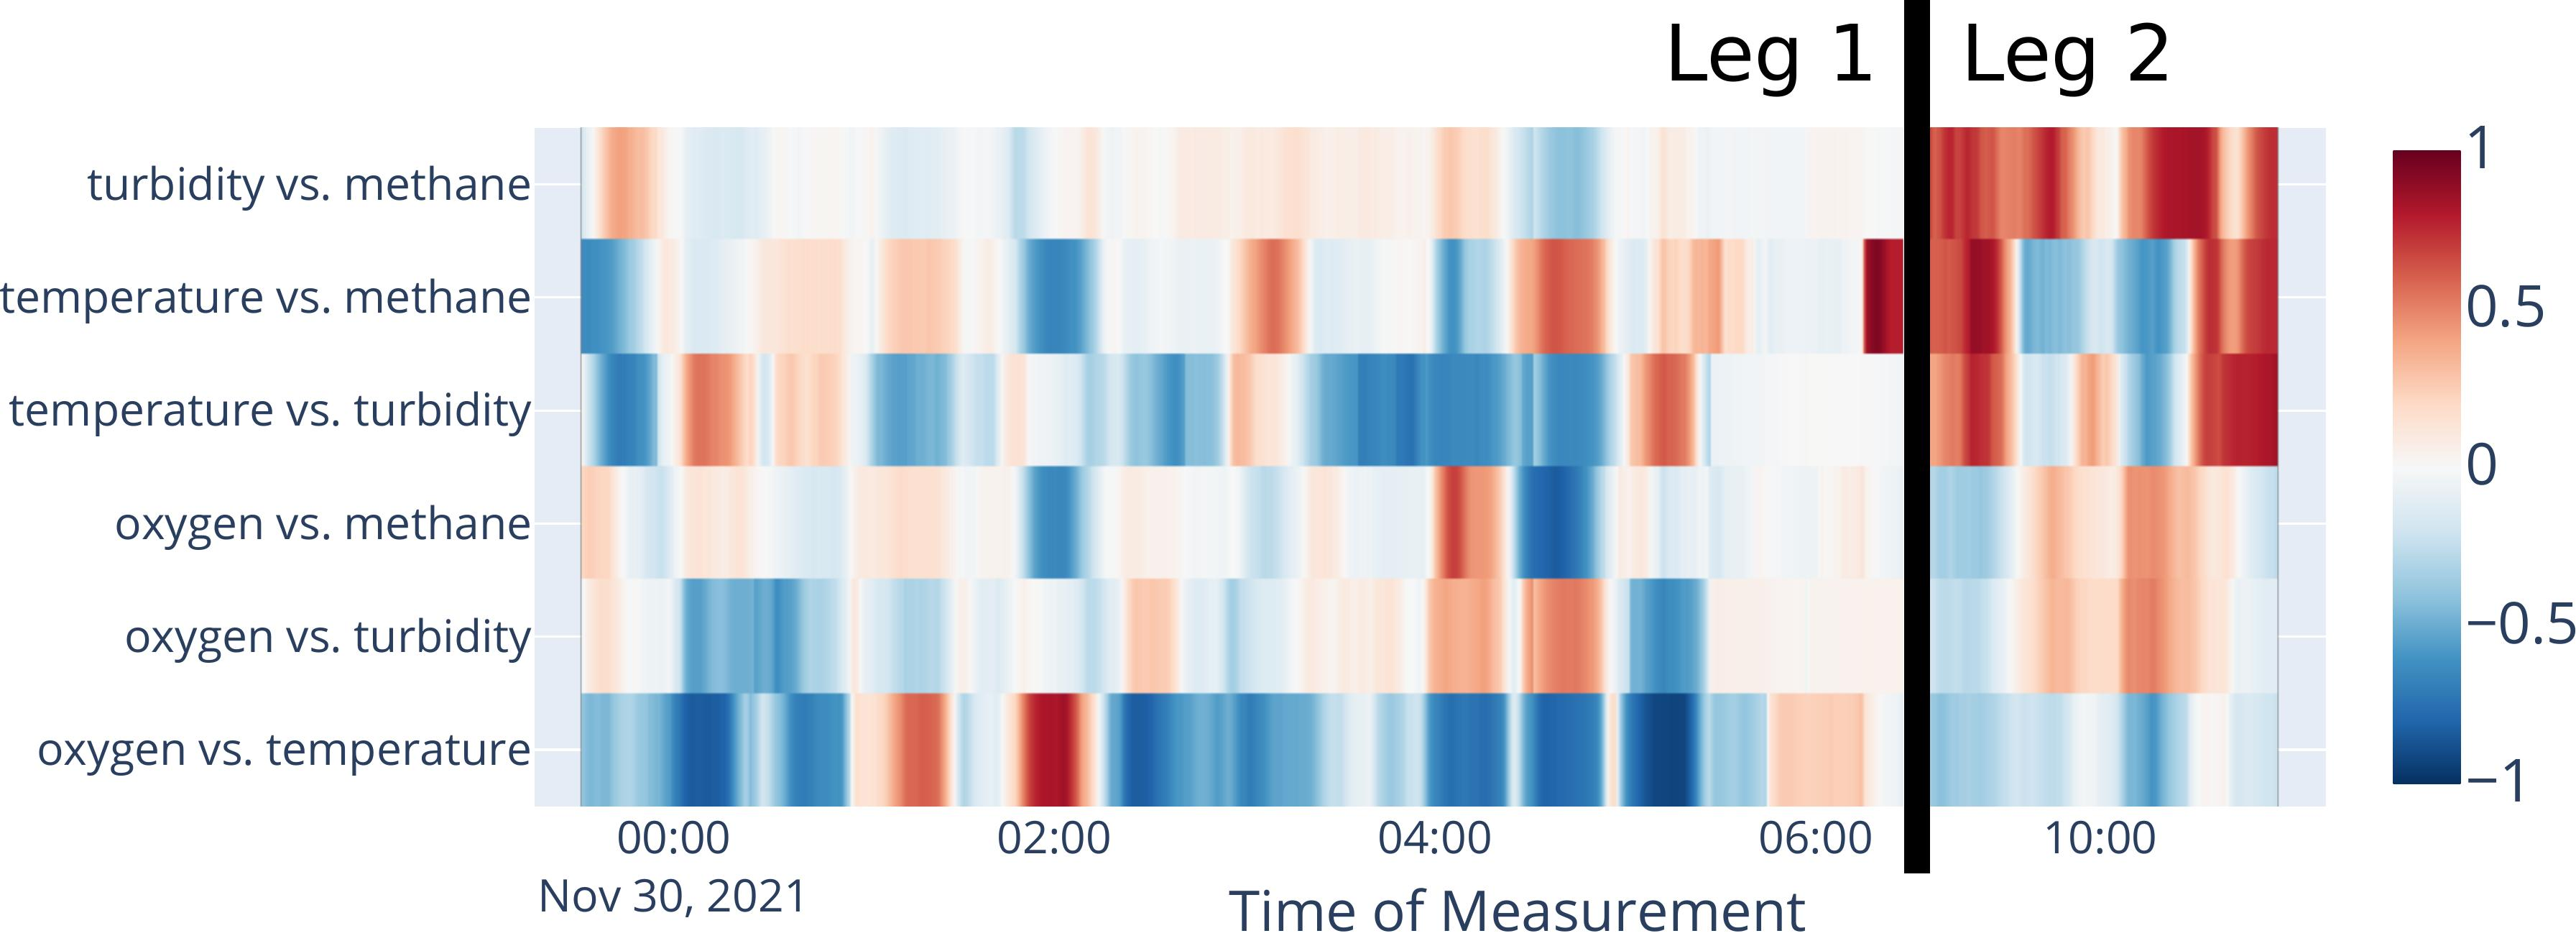
\includegraphics[width=\columnwidth]{figures/chap3_rosette_local_corr_all.jpg}
    \caption[Local (rolling) Pearson correlation coefficients for rosette mounted instruments.]{\textbf{Local (rolling) Pearson correlation coefficients between sensors mounted on the rosette over 30 minute windows.} Several regions of interest at 2:00 (strong temperature-oxygen correlation), 4:00-5:00 (notably coherent region of stronger correlation across multiple sensors), and during Leg 2 (near the venting source) can be picked out and may indicate anomalous water masses.}
    \label{fig:rosette_local}
\end{figure}

Local correlation trends during the \emph{Sentry} transect are reported in Fig.~\ref{fig:sentry_local}, and show an intense relationship between oxygen and temperature throughout the dive, with most of the transect reporting a strong negative correlation, save for two regions of positive correlation at 08:00 and again at 11:00. This strong relationship is also reflected in the relationships of temperature and oxygen with methane, being nearly correlative mirrors with respect to methane. During periods in which the turbidity sensor was operational, a gradual correlative ``flip'' and intensity increase in correlation between turbidity and oxygen around 11:00 may indicate a structured water mass. This time stamp agrees with the spatial proximity of \emph{Sentry} with the reference source.

\begin{figure}[h!]
    \centering
    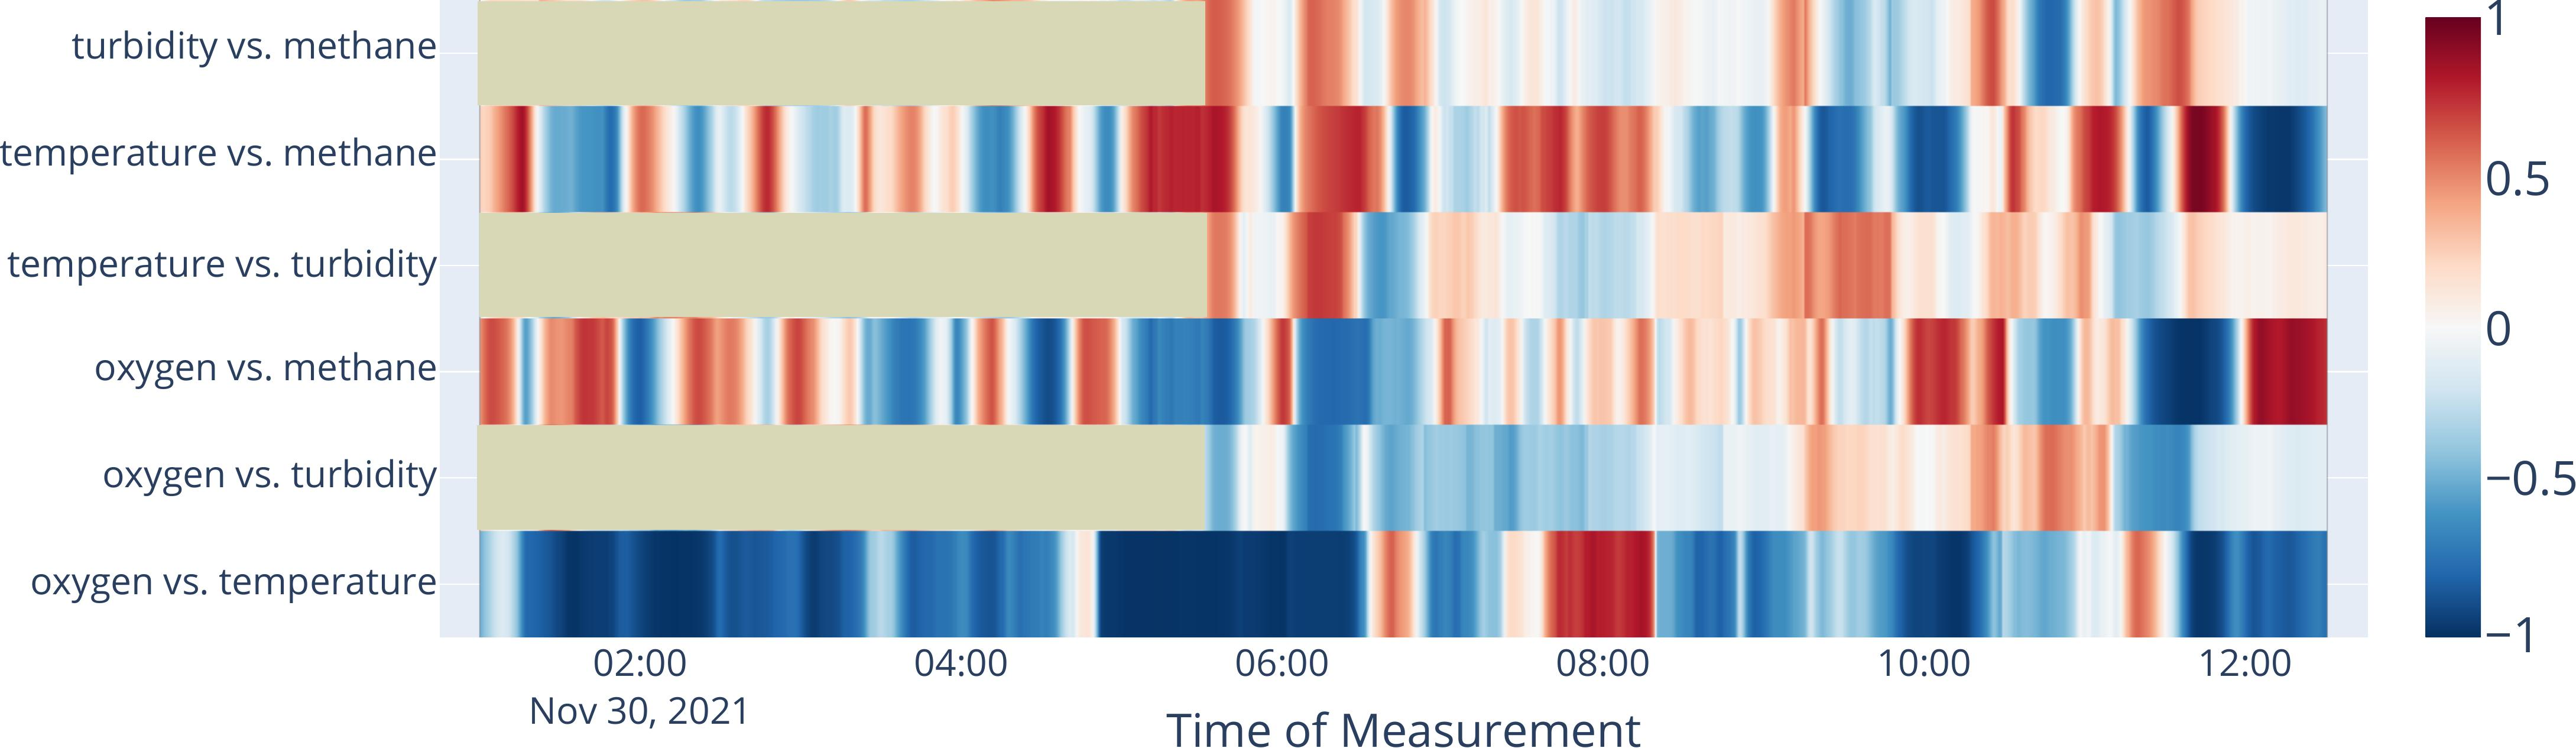
\includegraphics[width=1\columnwidth]{figures/chap3_sentry_local_corr_all.jpg}
    \caption[Local (rolling) Pearson correlation coefficients for AUV \Sentry mounted instruments.]{\textbf{Local (rolling) Pearson correlation coefficient between sensors mounted on AUV \emph{Sentry} over 30 minute windows.} Temperature and oxygen are strongly negatively correlated throughout the dive, with the exception of 08:00 and 11:00. For times in which the turbidity sensor was operational, the oxygen-turbidity correlative relationship slowly flips from negative to positive, with a peak positive correlation at 11:00. 11:00 agrees with the time that \Sentry was near the reference source vent.}
    \label{fig:sentry_local}
\end{figure}

Correlation alone is not sufficient evidence for the presence of hydrothermal fluids. For instance, some of the coherent regions of positive or negative correlation with methane any time during Leg 1, or early in the \emph{Sentry} transect, are misleading, as the overall methane content of the water was exceedingly small or essentially background. Rolling correlations, coupled with absolute thresholds as reported in \cref{sec:afar_results}, may together be useful tools for indicating transition into new water masses, their absolute properties of which could be used to more closely classify the types of water masses. This correlative study also demonstrates that correlations in expectation (e.g., temperature and methane being positively correlated in hydrothermal fluid) may be reductive assumptions of the complexities of plume evolution within a water column, supporting similar findings e.g., by~\cite{cowen2002methane}. For instance, aging plume waters in the neutrally buoyant layer may long have settled to a temperature indistinguishable from background, but still be particulate and possibly gas rich. This motivates additional study of the ``classes'' of hydrothermal fluids and their classifying characteristics, which could in turn be used to support studies of microbial evolution and nutrient consumption in plume fluids, or sediment and particulate transport modeling.

\subsection{Hydrothermalism Detection via Time-Series Regimes}
As indicated by Sec.~\ref{sec:correl}, changes in correlative \emph{structure} may be a more useful signal than absolute correlation alone. This notion can be codified as regime changes, which detect inflection points for which a series of observations collected in time may change in typical value, oscillation frequency, or pattern. Here, regime changes are computed over 30 minute detection windows using linearly penalized segmentation \autocite{killick2012optimal} (PELT) as implemented in the \verb|ruptures| Python library \autocite{truong2020selective} with a radial basis function detection kernel.
PELT is a linear-time offline algorithm for selecting changepoints that incrementally performs binary segmentation on a time-series (based on a cost function defined by the detection window and basis function) until all segments are self-consistent; these segments are regimes. In the included figures, we visualize regimes using alternating red and blue color blocks.

In Fig.~\ref{fig:rosette_regimes} regimes across the entire rosette transect over multiple sensors is illustrated. One initial observation is that the water-mixing anomaly that occurs early in the transect (Sec.~\ref{sec:o2_temp_salt}) appears to be detected as regime changes in potential temperature, oxygen, and even a correspondence in lowered beam attenuation. Similarly, regime changes in turbidity and methane are early indicators of significant elevation of both of these factors as the rosette intersects with hydrothermal fluids later in the transect. Interestingly, a regime change in oxygen and temperature is evident immediately following the first small peak in methane and turbidity in the absolute measurement data. These peaks, in addition to these regime changes, may together be indicative of mixing plume sources from other hydrothermal vents located along the ridge (that must travel further than fluids from our reference point) or the mixing of aging plume waters with more recently emitted fluids.

\begin{figure}[h!]
    \centering
    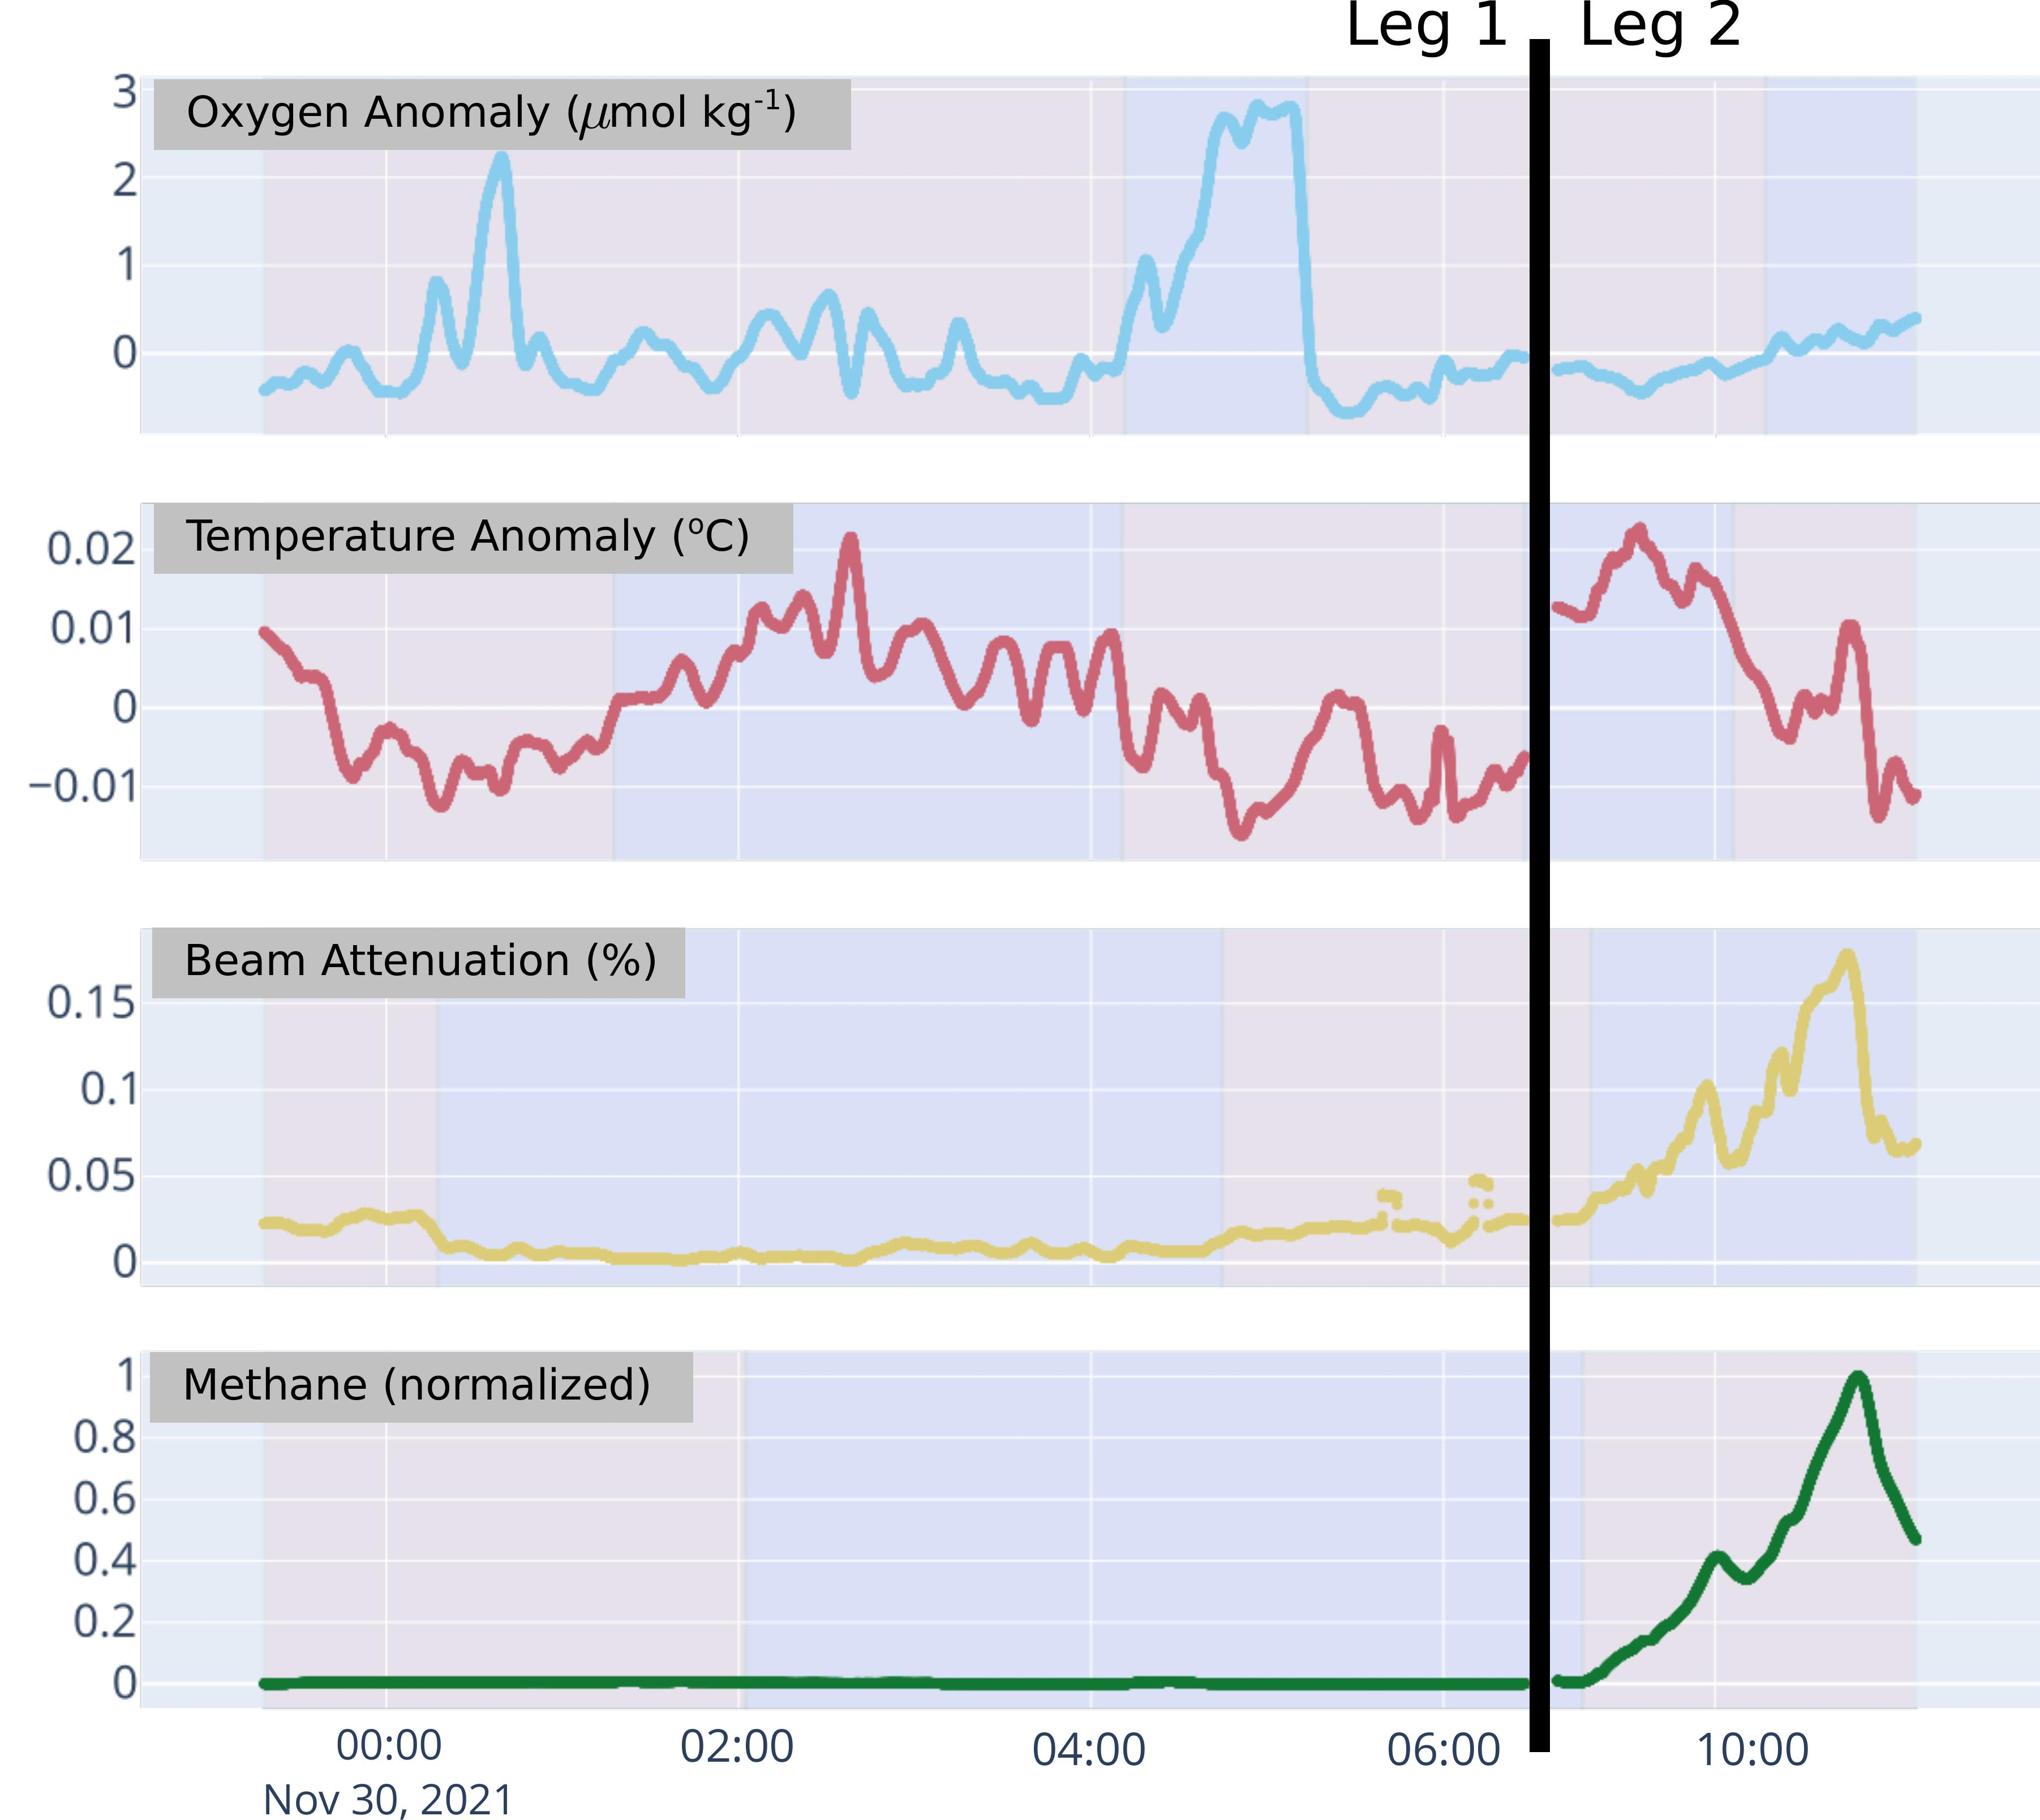
\includegraphics[width=1\columnwidth]{figures/chap3_rosette_regimes.jpg}
    \caption[Regime changes in rosette observations.]{\textbf{Regime changes in rosette observations.} Regimes, indicated as alternating blue and red regions, detected during the rosette transect with a 30 minute detection window.}
    \label{fig:rosette_regimes}
\end{figure}


With instruments mounted on \emph{Sentry}, in Fig.~\ref{fig:sentry_regimes}, clear ``steps'' of methane observed by Pythia each mark a regime in that data stream. Some of these steps are nearly coincident with regime changes in turbidity, temperature, and oxygen (particularly the steps at 06:30 and 09:30).  

\begin{figure}[h!]
    \centering
    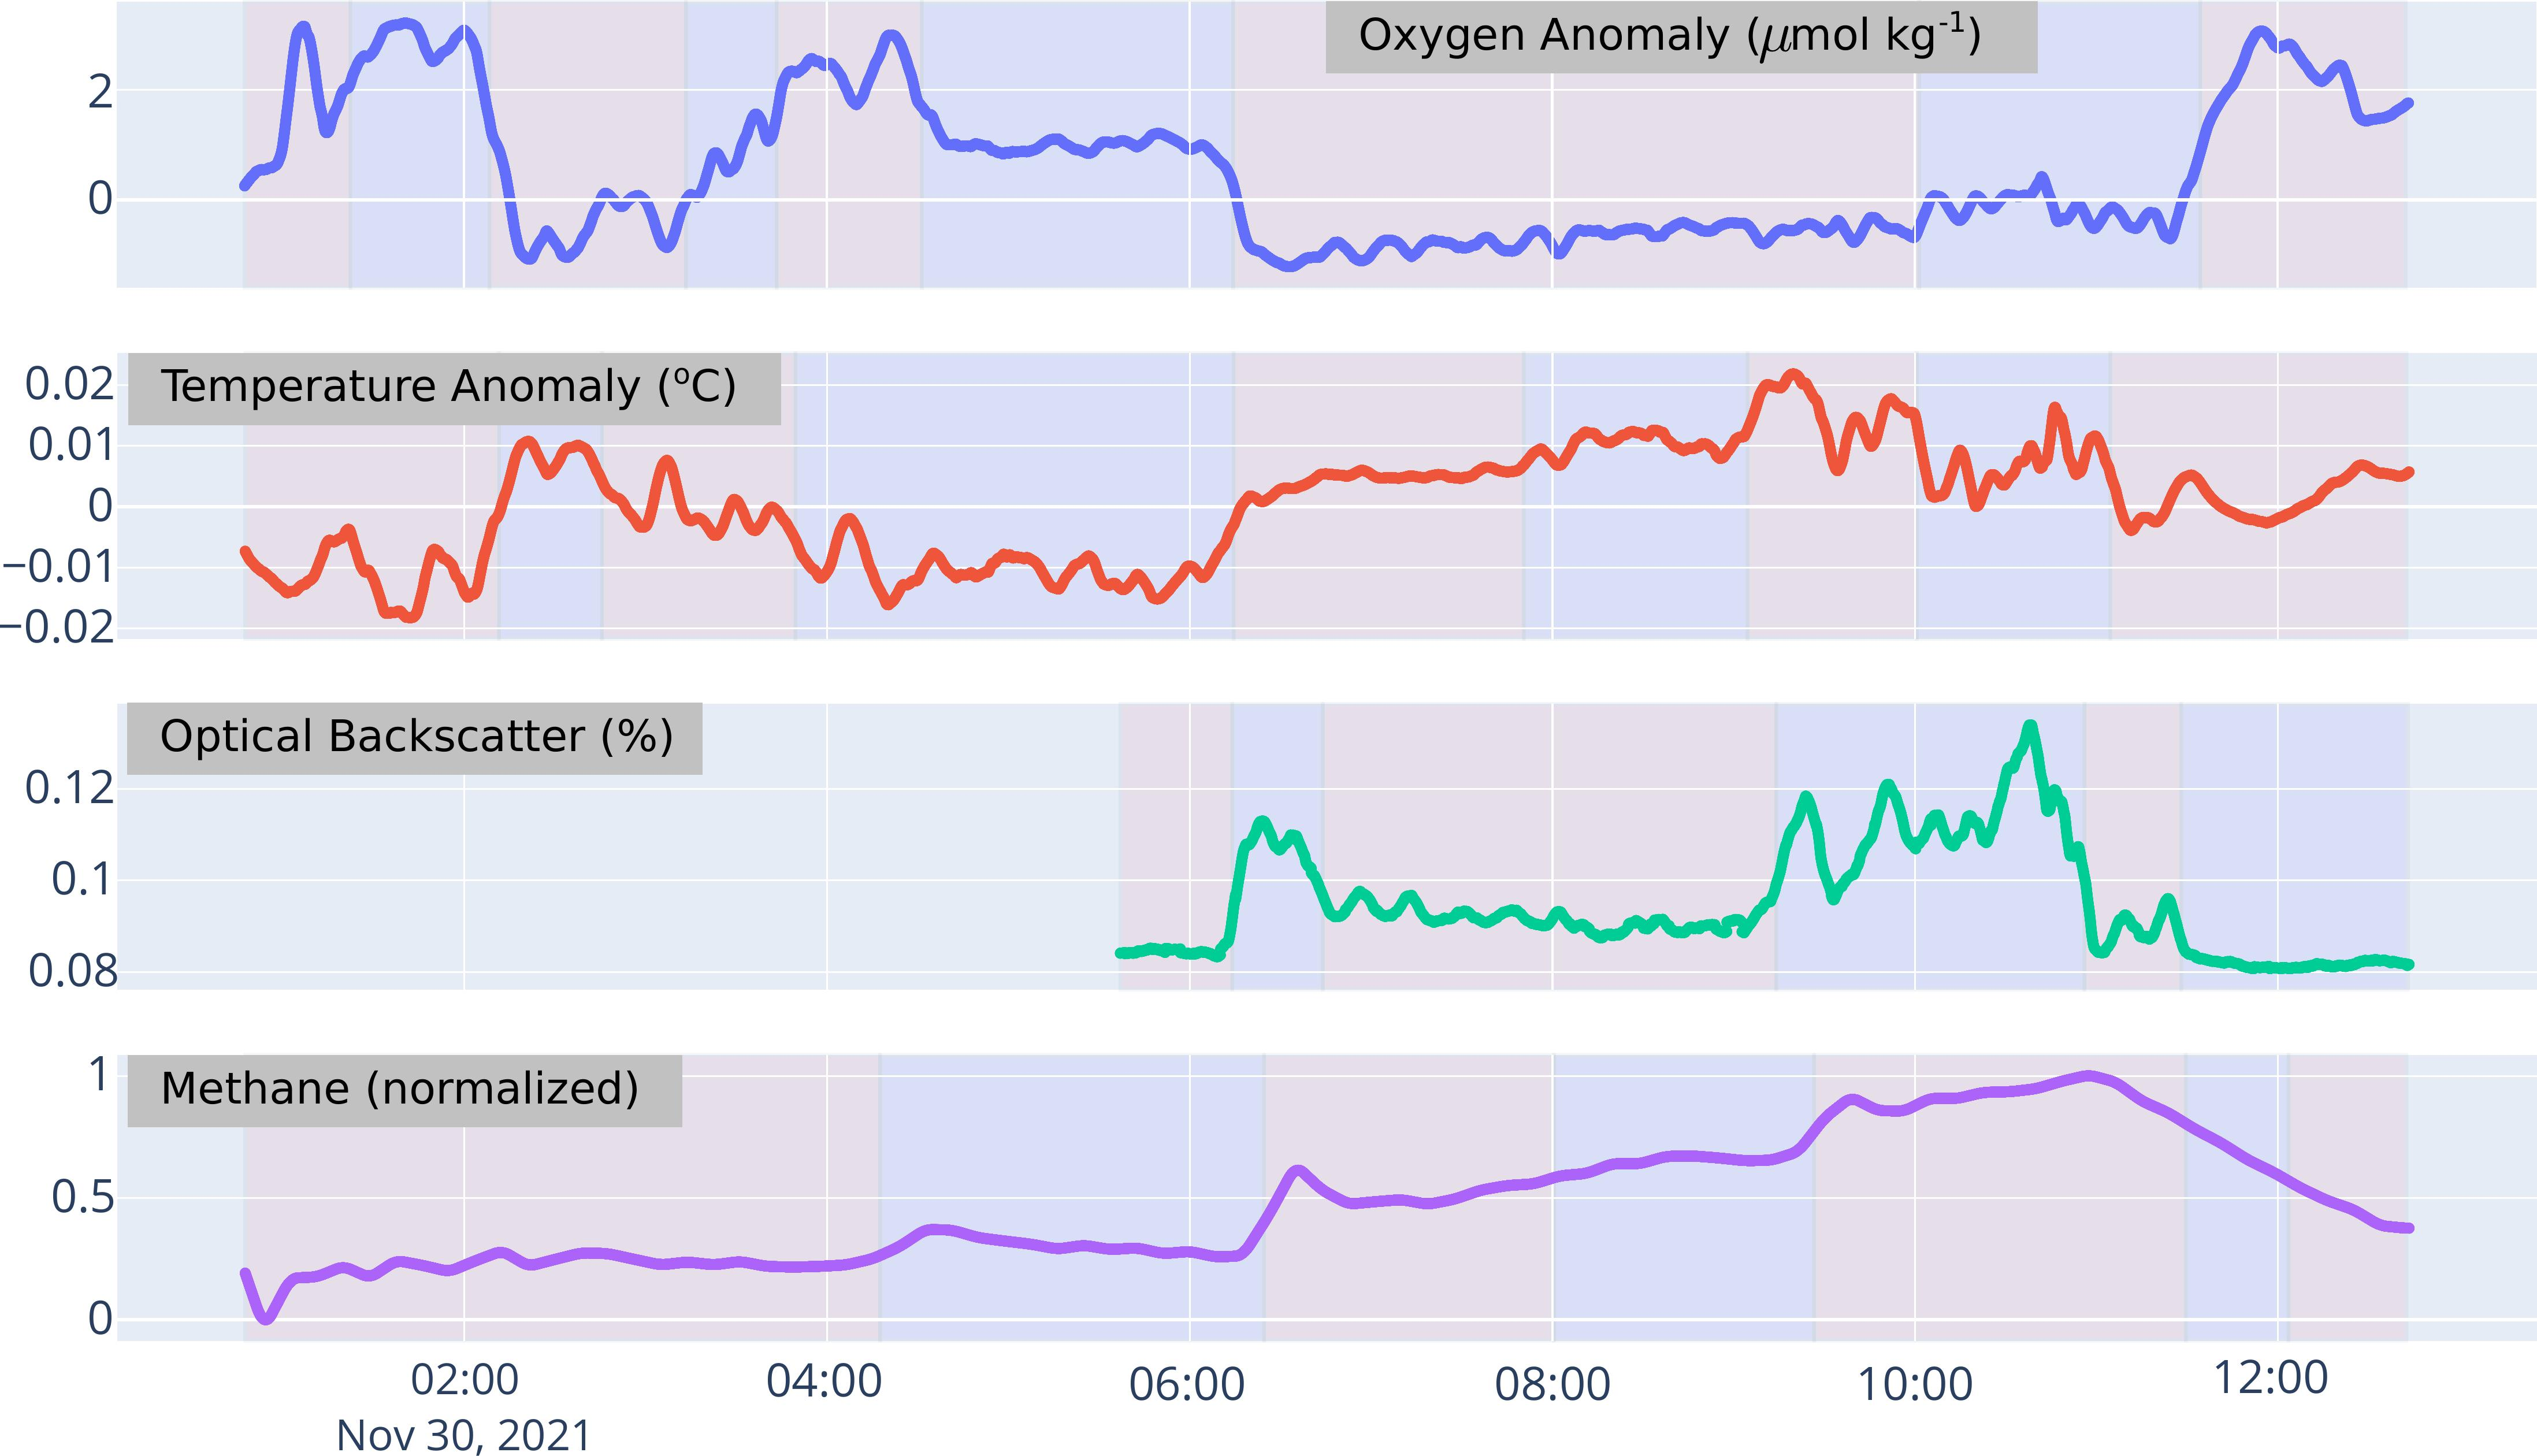
\includegraphics[width=1\columnwidth]{figures/chap3_sentry_regimes.jpg}
    \caption[Regime changes in AUV \Sentry observations.]{\textbf{Regime changes in AUV \Sentry observations.} Regimes, indicated as alternating blue and red regions, detected during the AUV \emph{Sentry} transect with a 30 minute detection window.}
    \label{fig:sentry_regimes}
\end{figure}

Regimes can be mathematically identified in streaming data, making this a potentially useful method to adopt for real-time hydrothermalism discovery. Coupled with absolute measurements by sensing instruments and rolling correlative structure, identifying water masses across multiple data streams can be done live from streaming data on the ship. The simplicity of the computation and the nature of these analysis techniques as data reduction methods (e.g., regimes can be reported as a single time stamp; cross-correlations over strategic sensor pairs could be reported as a single float) additionally make computing these measures onboard an AUV and reporting them back to watchstanders under data-limited transmission protocols (e.g., acoustic pings) feasible. 


\subsection{Methane in Deep Sea Exploration}
AUV and sensor deployments during expedition RR2107 served as an initial proving ground for the SAGE and Pythia \emph{in situ} methane instruments for deep sea exploration, and the utility of methane as a potential tracer for hydrothermalism discovery. During this transect both instruments observed significantly elevated methane over a span of several kilometers from a known hydrothermal source in Guaymas Basin. Methane proved to be a strong predictor for hydrothermalism that was not easily confounded by physical oceanographic events (e.g., mixing), giving it an advantage over oxygen, temperature, and salinity. Indeed, in this trial, each of the oxygen, temperature, and salinity instruments were impacted by an unknown physical feature not driven by hydrothermalism, but registered as similar scales of expected anomaly. Methane was also shown to be more expressive than ORP, which only registered a possible anomaly long after significant methane measurements were observed. Turbidity was a similarly useful and expressive feature of hydrothermalism in this basin, with similar detection scales to methane during this transect. Notably, for less strict detection criteria (i.e., thresholds) on detection, methane significantly outperformed turbidity in terms of detection scale (positive identification up to 6.8 km away, in contrast to 3.4 km for turbidity). Turbidity and methane together make for a strong pairing for hydrothermalism discovery. While neither one alone is a ``universal'' proxy for hydrothermal activity---not all hydrothermalism of interest produces particulate heavy smoke (i.e., diffuse flow fields) nor do all vents produce significantly elevated methane---they are complementary indicators which can assist in deep sea exploration for anomalous water masses derived from hydrothermalism. 

Collecting high resolution measurements of methane during this transect highlighted the rich structure of dissolved gasses in a neutrally buoyant plume layer over multiple kilometers, with multiple peak detections being possibly indicative of mixing novel and aging hydrothermal fluids, the contribution of multiple sources of hydrothermalism, or complicated internal mixing causing spatiotemporal multimodal distributions of dissolved gas ``pockets'' throughout the layer. Bottle samples collected on the research cruise verified the presence and general trend of methane observed by the instruments, but failed to resolve several features that may be of scientific interest. This motivates the use of \emph{in situ} methane sensors for future studies of hydrothermal fluids in the water column. 


\subsection{Enabling Better Decision-Making for Hydrothermalism Discovery}
Enabling the interpretation of real-time sensor data and adapting scientific missions accordingly are critical future skills for scientific expeditions and exploration in the deep sea. In preparation for this transect, a simple physical model was used to inform the design of the trajectory and monitored progress with live data displays for both the rosette and AUV \emph{Sentry}. While real-time data display for rosettes is now considered standard for oceanographic research, streaming capabilities of scientific data from autonomous platforms like \emph{Sentry} is a relatively new capability. This display infrastructure enabled the science team to make note of the OBS sensor error on \emph{Sentry} while performing the transect, caught a power and logging failure of the Pythia logger upon deployment (which, if left unresolved, would have meant an absence of all methane data associated with \emph{Sentry} for this analysis), and made real-time control and decision-making about the rosette positioning and bottle firing possible. While data presented here was analyzed after the mission, several of these analyses, including rolling correlation and regime detection, could be performed from streaming observations. As a whole, the techniques in this chapter present an opportunity for advancing technical infrastructure on a research vessel in order to enhance decision-making capabilities of the science party and engineering teams, both logistically to better diagnose instrument operation \emph{in situ} and scientifically to enhance data collection.

Real-time data collection and processing could have further implications for embodied intelligence as a tool for scientific expeditions. Using models, inference methods, and streaming data, autonomous agents like AUV \emph{Sentry} could be made capable of performing adaptive decision-making for sample collection. Hydrothermalism discovery has long been a motivating use case for intelligent autonomy at sea \autocite{yoerger2007autonomous, jakuba2007stochastic, branch2020demonstration, wang20203}. This transect experiment demonstrates the utility of simple models for tractable, intelligent planning, motivates the possibility of using methane as an additional, reliable data source for performing autonomous behaviors (e.g., adaptive sampling, tracking), and presents the opportunity to embed simple analytical methods for classifying hydrothermal fluids from sensor streams. Being able to both map the source of hydrothermal plumes with ROVs and chart the evolving nature of fluids in the mid-water with AUVs, would enable an advancement of scientific inquiries that could be pursued with respect to hydrothermalism in the deep ocean. Such queries include the detailed structure of multiple-source plume collision, directly measuring \emph{in situ} the 4D structure of mixing in neutrally buoyant plumes and buoyant plume stems, assessing biological activity supported by plume fluids, tracing the fate of dissolved gasses, and more. This work demonstrates that detection of hydrothermal sources is possible on the scale of several kilometers even from relatively small hydrothermal vents that are present in Guaymas Basin, and has taken initial steps to demonstrate core data infrastructure that can improve human decision-making in hydrothermalism discovery; future work and engagement will be focused on advancing these tools to enable the next generation of scientific inquiry in the deep ocean.
